\thispagestyle{toancuabinone}
\pagestyle{toancuabi}
\everymath{\color{toancuabi}}
\blfootnote{$^1$\color{toancuabi}Trường Liên cấp Hội nhập Quốc tế iSchool Quảng Trị.}
\graphicspath{{../toancuabi/pic2/}}
\begingroup
\AddToShipoutPicture*{\put(0,616){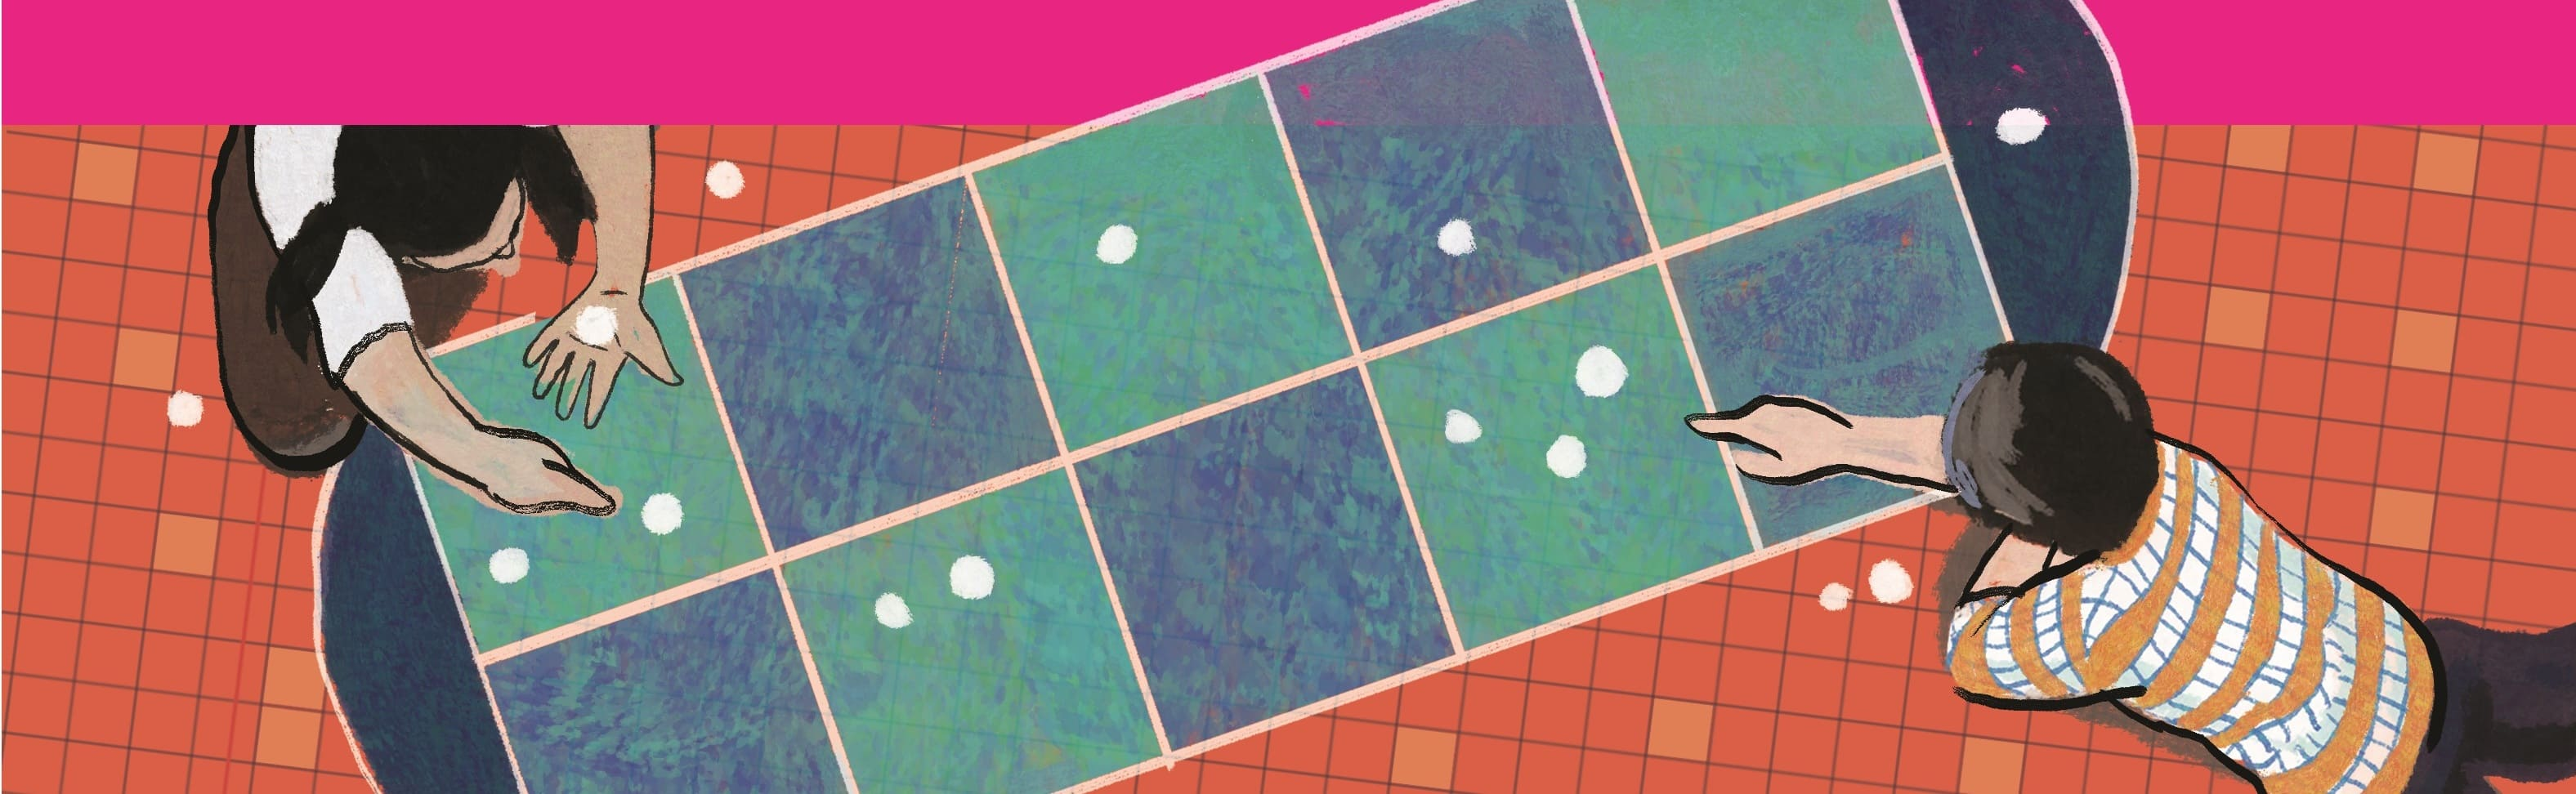
\includegraphics[width=19.3cm]{../bannertoancuabi}}}  
\AddToShipoutPicture*{\put(48,552){
\includegraphics[scale=1]{../tieude10.pdf}}}  
\centering
\endgroup
\vspace*{155pt} 

%\begin{multicols}{2}
%	\textbf{\color{toancuabi}Gấp trái tim bằng giấy}
%	\vskip 0.1cm
%	Các em chỉ cần chuẩn bị một tờ giấy màu hình vuông. Sau đó hãy làm theo các bước chỉ dẫn như sau là đã có được một trái tim xinh xắn bằng giấy rồi!
%	\vskip 0.1cm
%	\textit{Bước} $1$: Gấp đôi tờ giấy hình vuông $2$ lần để tạo nếp. 
%	\begin{figure}[H]
%		\vspace*{-5pt}
%		\centering
%		\captionsetup{labelformat= empty, justification=centering}
%		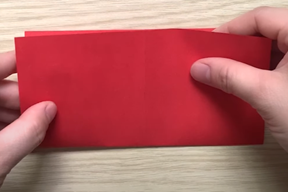
\includegraphics[height= 0.327\linewidth]{20}
%		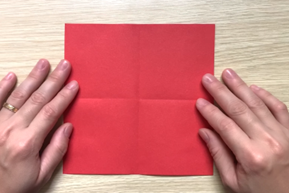
\includegraphics[height= 0.327\linewidth]{21}
%		\vspace*{-10pt}
%	\end{figure}
%	\textit{Bước} $2$: Gấp $\dfrac{1}{4}$ tờ giấy lên phía trên chạm vào chính giữa tờ giấy. Dùng tay miết nhẹ để tạo nếp gấp.
%	\begin{figure}[H]
%		\vspace*{-5pt}
%		\centering
%		\captionsetup{labelformat= empty, justification=centering}
%		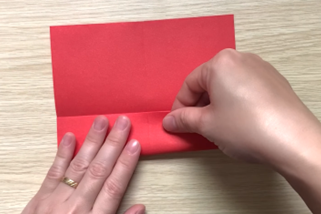
\includegraphics[width= 1\linewidth]{22}
%		\vspace*{-15pt}
%	\end{figure}
%	Bước $3$: Lật mặt sau tờ giấy lại rồi gấp như các hình minh họa bên dưới. 
%	\begin{figure}[H]
%		\vspace*{5pt}
%		\centering
%		\captionsetup{labelformat= empty, justification=centering}
%		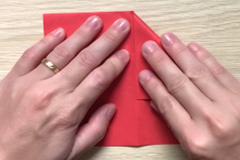
\includegraphics[height= 0.327\linewidth]{23}
%		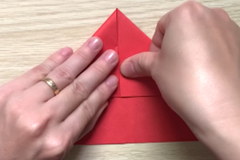
\includegraphics[height= 0.327\linewidth]{24}
%		
%		\vspace*{1pt}
%		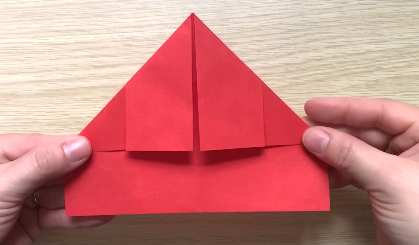
\includegraphics[width=1\linewidth]{25}
%		\vspace*{-15pt}
%	\end{figure}
%	\textit{Bước} $4$: Tiếp tục lật mặt sau tờ giấy lại rồi gấp như hình minh họa. 
%	\begin{figure}[H]
%		\vspace*{-5pt}
%		\centering
%		\captionsetup{labelformat= empty, justification=centering}
%		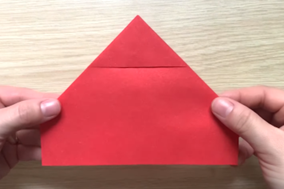
\includegraphics[height= 0.327\linewidth]{26}
%		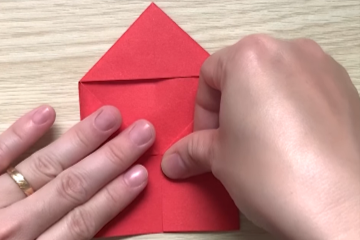
\includegraphics[height= 0.327\linewidth]{27}
%		
%		\vspace*{1pt}
%		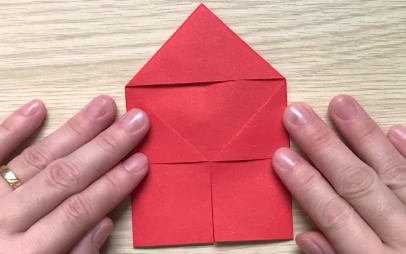
\includegraphics[width=1\linewidth]{28}
%		\vspace*{-10pt}
%	\end{figure}
%	\textit{Bước} $5$: Gấp hai góc phía dưới lên.
%	\begin{figure}[H]
%		\vspace*{-5pt}
%		\centering
%		\captionsetup{labelformat= empty, justification=centering}
%		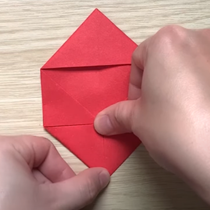
\includegraphics[height= 0.485\linewidth]{29}
%		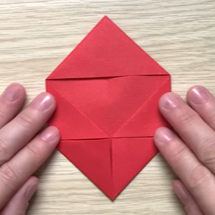
\includegraphics[height= 0.485\linewidth]{30}
%		\vspace*{-10pt}
%	\end{figure}
%	\textit{Bước} $6$: Gấp đôi hình lại sao cho phần nhọn của tam giác phía dưới trùng khớp với phần nhọn của tam giác phía trên. Dùng tay miết nhẹ để tạo nếp gấp rồi mở ra.
%	\begin{figure}[H]
%		\vspace*{-5pt}
%		\centering
%		\captionsetup{labelformat= empty, justification=centering}
%		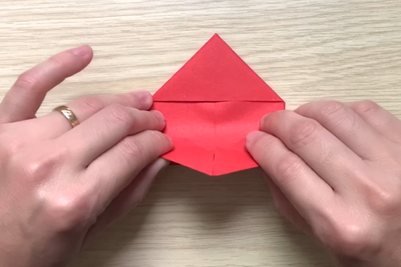
\includegraphics[width=0.65\linewidth]{31}
%		
%		\vspace*{1pt}
%		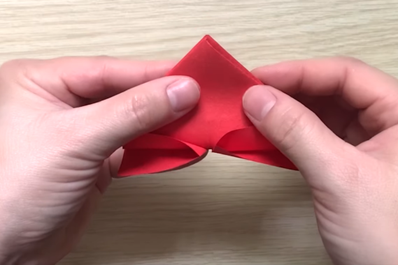
\includegraphics[width=0.65\linewidth]{32}
%		\vspace*{-10pt}
%	\end{figure}
%	\textit{Bước} $7$: Luồn phần nhọn của tam giác phía dưới vào kẽ hở của tam giác phía trên.
%	\begin{figure}[H]
%		\vspace*{-5pt}
%		\centering
%		\captionsetup{labelformat= empty, justification=centering}
%		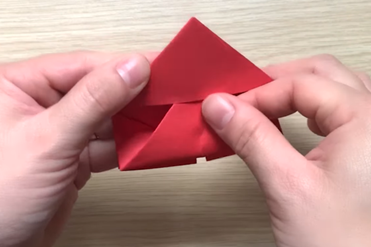
\includegraphics[width=0.65\linewidth]{33}
%		
%		\vspace*{1pt}
%		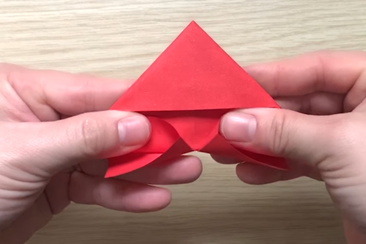
\includegraphics[width=0.65\linewidth]{34}
%%		\vspace*{-10pt}
%	\end{figure}
%	\vskip 0.1cm
%	\columnbreak
%	\textit{Bước} $8$: Gấp hai góc nhỏ như hình minh họa.
%	\begin{figure}[H]
%		\vspace*{-5pt}
%		\centering
%		\captionsetup{labelformat= empty, justification=centering}
%		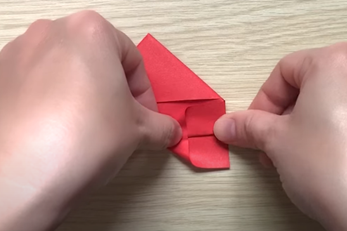
\includegraphics[height= 0.327\linewidth]{35}
%		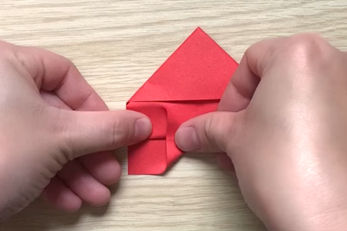
\includegraphics[height= 0.327\linewidth]{36}
%		
%		\vspace*{1pt}
%		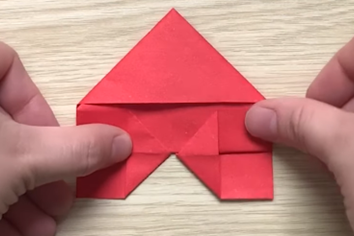
\includegraphics[height= 0.327\linewidth]{37}
%		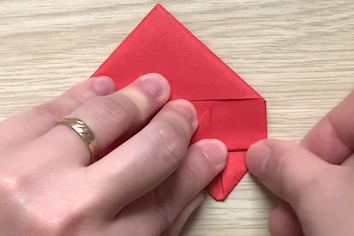
\includegraphics[height= 0.327\linewidth]{38}
%		
%		\vspace*{1pt}
%		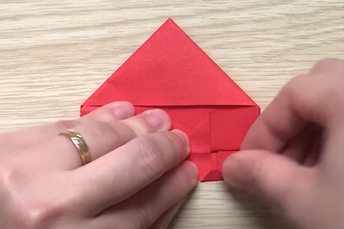
\includegraphics[height= 0.327\linewidth]{39}
%		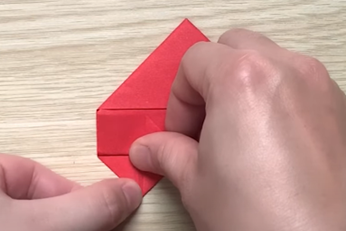
\includegraphics[height= 0.327\linewidth]{40}
%		
%		\vspace*{1pt}
%		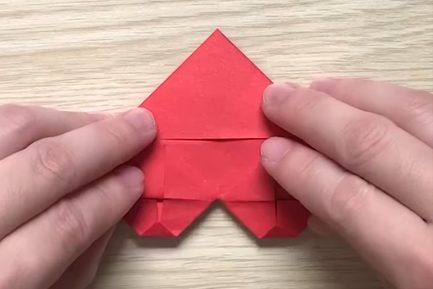
\includegraphics[height= 0.327\linewidth]{41}
%		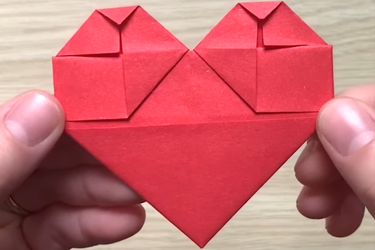
\includegraphics[height= 0.327\linewidth]{42}
%		
%		\vspace*{1pt}
%		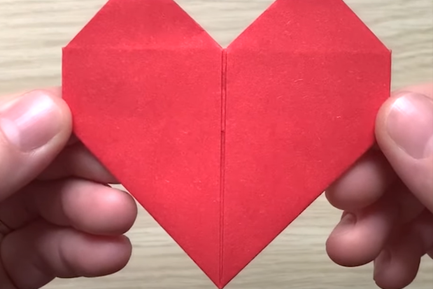
\includegraphics[width=1\linewidth]{43}
%		\vspace*{-15pt}
%	\end{figure}
%	Như vậy là chúng ta đã hoàn thành xong việc gấp trái tim bằng giấy rồi. Trái tim bằng giấy em vừa gấp xong có bao nhiêu trục đối xứng vậy?
%	\begin{figure}[H]
%		\vspace*{-5pt}
%		\centering
%		\captionsetup{labelformat= empty, justification=centering}
%		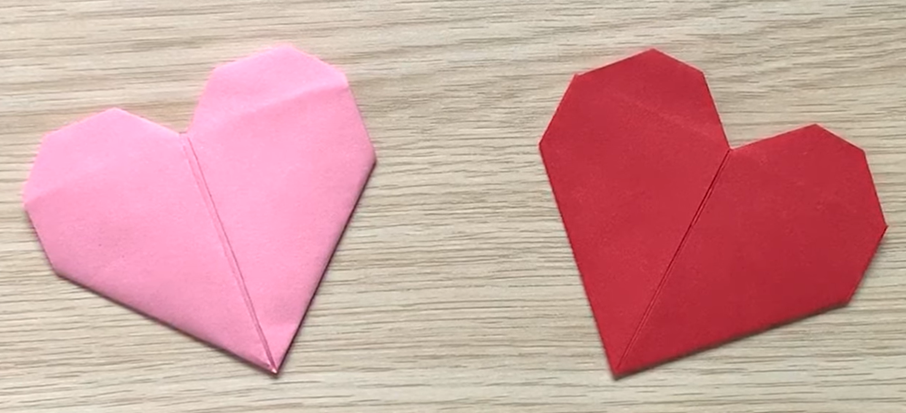
\includegraphics[width= 1\linewidth]{44}
%		\vspace*{-15pt}
%	\end{figure}
%	
%	
%\end{multicols}

%\begin{multicols}{2}
%	Thám tử Xuân Phong cùng thanh tra Lê Kính tham gia một buổi giới thiệu sản phẩm của hai công ty là Tae Yeon và Tea Yon tại triển lãm Điện tử Expo -- New Vision của khu vực. Công ty  Tae Yeon có uy tín từ lâu đời, với những sản phẩm tinh tế có chất lượng tốt nổi tiếng,  các nhân viên của công ty luôn nói thật. Còn công ty Tea Yon chuyên sản xuất đồ rẻ, kém chất lượng, bắt chước kiểu dáng của công ty Tae Yeon nên Ban giám đốc dặn các nhân viên của mình chỉ được nói dối trong buổi triển lãm. 
%	\vskip 0.1cm
%	Vừa đặt chân tới khu vực triển lãm được trang hoàng lộng lẫy, Xuân Phong gặp ngay $5$ đại diện  của hai công ty này đứng tại cổng ra vào và tươi cười niềm nở tiếp đón. Xuân Phong tiến tới họ và hỏi cả $5$ người cùng một câu hỏi ``Có bao nhiêu người đến từ công ty Tae Yeon trong số các bạn?" 
%	\vskip 0.1cm
%	Người thứ nhất trả lời ``Không có ai cả". Hai người tiếp theo đều trả lời ``Có đúng một người". 
%	\vskip 0.1cm
%	Vậy hai người còn lại sẽ trả lời câu hỏi của thám tử Xuân Phong như thế nào nhỉ? Em có thể suy đoán ra câu trả lời của họ và giải thích lập luận được không?
%	\begin{figure}[H]
	%		\centering
	%		\vspace*{-5pt}
	%		\captionsetup{labelformat= empty, justification=centering}
	%		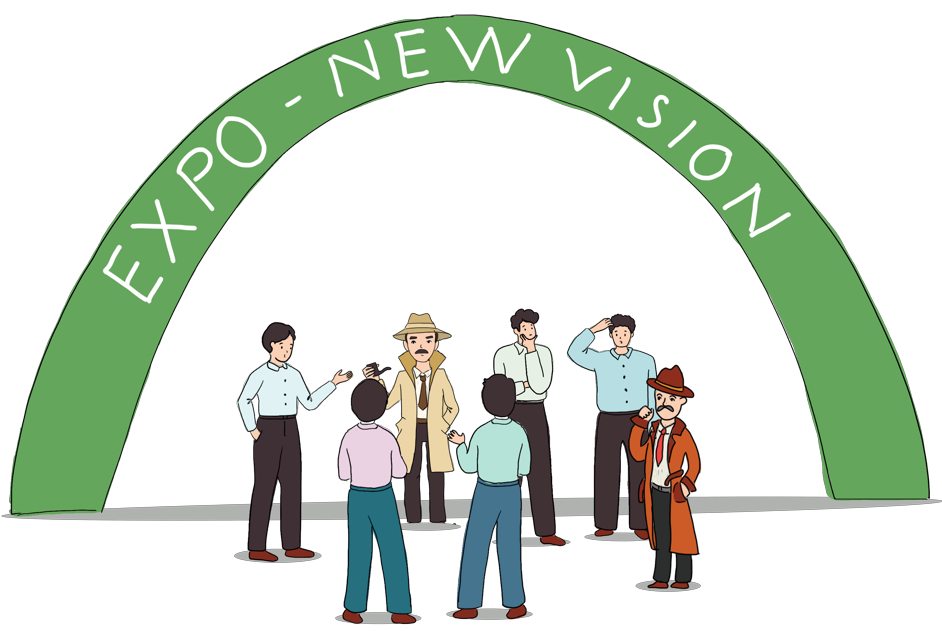
\includegraphics[width=1\linewidth]{xuanphong}
	%		\vspace*{-5pt}
	%	\end{figure}
%\end{multicols}
%\vspace*{-10pt}
%{\color{toancuabi}\rule{1\linewidth}{0.1pt}}
%\begingroup
%\AddToShipoutPicture*{\put(115,190){
\includegraphics[scale=1]{../tieude11.pdf}}} 
%\centering
%\endgroup
%\vspace*{50pt}
%
%\begin{multicols}{2}
%	$\pmb{1.}$	Trong một cuộc thi thể thao, ban tổ chức chọn ra một số bạn học sinh ở lớp $5A$ và một số bạn ở lớp $5B$ thi đấu trực tiếp. Mỗi bạn ở lớp $5A$ được chọn ra sẽ thi đấu duy nhất một trận với một bạn ở lớp $5B$, và ngược lại, mỗi bạn ở lớp $5B$ được chọn ra chỉ đấu đúng một trận với một bạn ở lớp $5A$.
%	\begin{figure}[H]
	%		\centering
	%		\vspace*{-5pt}
	%		\captionsetup{labelformat= empty, justification=centering}
	%		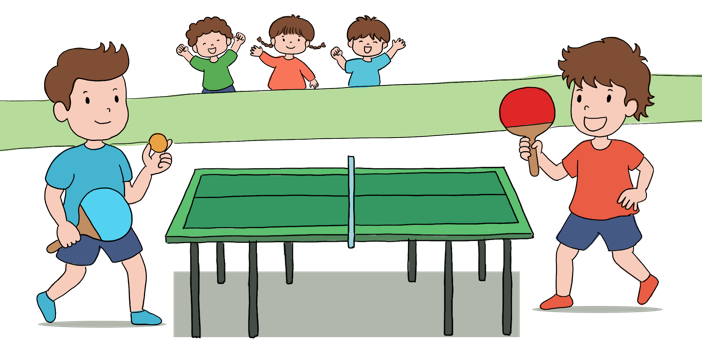
\includegraphics[width=1\linewidth]{Pi5_bai1}
	%		\vspace*{-15pt}
	%	\end{figure}
%	Biết rằng số học sinh lớp $5A$ được chọn thi đấu chiếm $2/3$ tổng số học sinh toàn lớp $5A$, còn số học sinh lớp $5B$ được chọn thi đấu chiếm $3/5$ tổng số học sinh toàn lớp $5B$. Tổng số học sinh của cả hai lớp là $57$ bạn. Hỏi có bao nhiêu học sinh của hai lớp đã tham gia các trận thi đấu trực tiếp?
%	
%	$\pmb{2.}$ Công ty vận tải được thông báo ngắn gọn là có một số kiện hàng có tổng khối lượng là $10$ tấn cần được vận chuyển, hơn nữa mỗi kiện hàng nặng không quá $1$ tấn. Hỏi công ty  cần điều động ít nhất bao nhiêu xe tải có trọng tải là $3$ tấn mỗi xe để luôn chắc chắn chở được hết được số hàng hoá đó?
%	\begin{figure}[H]
	%		\centering
	%		\vspace*{-10pt}
	%		\captionsetup{labelformat= empty, justification=centering}
	%		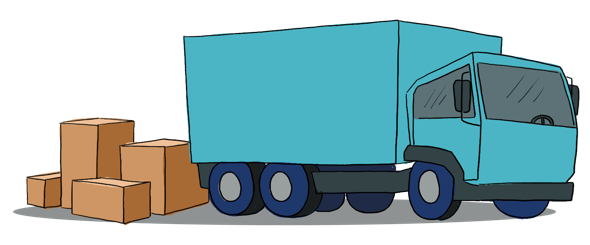
\includegraphics[width=0.8\linewidth]{Pi5_bai2}
	%		\vspace*{-15pt}
	%	\end{figure}
%	$\pmb{3.}$ Sau khi được sạc đầy pin, điện thoại di động của bạn An dùng đúng $6$ tiếng ở chế độ trò chuyện hoặc đúng $210$ tiếng ở chế độ chờ. Khi bạn An lên tàu hoả để đi du lịch, pin của bạn được sạc đầy $100\%$, và trên tàu không có ổ cắm sạc nên khi xuống ga, pin của bạn cũng vừa hết sạch. Biết rằng An đã nói chuyện với bạn bè đúng một nửa thời gian khi ngồi trên tàu, còn nửa thời gian còn lại đặt điện thoại ở chế độ chờ. Hỏi thời gian An đi trên tàu hoả là bao nhiêu lâu?
%	\begin{figure}[H]
	%		\centering
	%		\vspace*{-5pt}
	%		\captionsetup{labelformat= empty, justification=centering}
	%		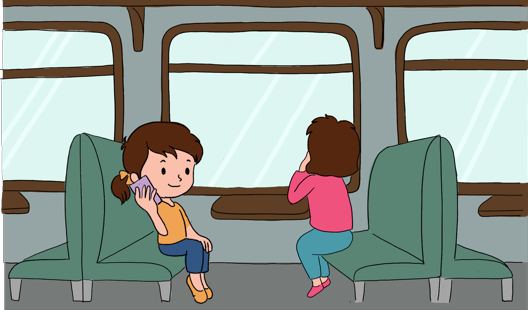
\includegraphics[width=0.85\linewidth]{Pi5_bai3}
	%		\vspace*{-10pt}
	%	\end{figure}
%	$\pmb{4.}$ Một nhóm học sinh đi bộ từ điểm hẹn tới bến xe buýt để kịp đón chuyến xe vào lúc $8$ giờ. Cũng vào thời điểm này, từ điểm tham quan, một chiếc xe buýt cũng xuất phát để tới kịp bến xe đón nhóm học sinh đó. Tuy  nhiên nhóm học sinh tới bến xe buýt khá sớm, vào lúc $6$ giờ $10$ phút, nên họ quyết định đi bộ tiếp tới điểm tham quan. Trên đường, các bạn đã gặp được xe buýt và lên xe đi tiếp.  Cuối cùng cả nhóm đến được điểm tham quan sớm hơn $20$ phút so với thời gian ấn định. Biết rằng vận tốc của xe buýt là $60$ km/h và vận tốc đi bộ của các em học sinh luôn không đổi. Hãy tìm vận tốc đi bộ của nhóm học sinh trước khi gặp xe buýt.
%	\begin{figure}[H]
	%		\centering
	%		\vspace*{-10pt}
	%		\captionsetup{labelformat= empty, justification=centering}
	%		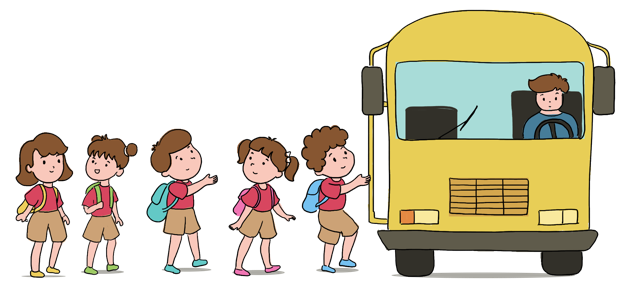
\includegraphics[width=0.85\linewidth]{Pi5_bai4}
	%		\vspace*{-10pt}
	%	\end{figure}
%	$\pmb{5.}$ 	Có $100$ chiếc xe ô tô đỗ liền nhau thành một hàng dọc bên lề đường, trong đó có $70$ chiếc xe hiệu Mercedes, còn lại là những xe nhãn hiệu khác. Trong các xe nhãn hiệu Mercedes có $30$ chiếc màu đỏ, $20$ chiếc màu vàng và $20$ chiếc màu hồng. Biết rằng không có hai xe Mercedes nào khác màu lại đỗ cạnh nhau. Em hãy chỉ ra rằng luôn tìm ra $3$ chiếc xe Mercedes cùng màu đỗ liên tiếp nhau.
%	\begin{figure}[H]
	%		\centering
	%		\vspace*{-5pt}
	%		\captionsetup{labelformat= empty, justification=centering}
	%		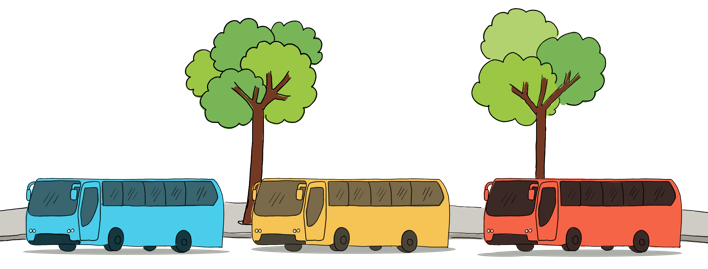
\includegraphics[width=0.85\linewidth]{Pi5_bai5}
	%		\vspace*{-10pt}
	%	\end{figure}
%	$\pmb{6.}$ Một lớp học có $20$ em học sinh. Cô giáo chủ nhiệm của lớp tổ chức một số buổi tham quan vào mỗi ngày cuối tuần trong suốt năm học, mỗi buổi tham quan có ít nhất $4$ em học sinh tham gia. Em hãy chứng minh rằng có một buổi tham quan mà mỗi em học sinh tham gia buổi đó đều tham gia ít nhất $1/17$ tổng số tất cả các buổi tham quan của cả năm học.
%	\begin{figure}[H]
	%		\centering
	%		\vspace*{-15pt}
	%		\captionsetup{labelformat= empty, justification=centering}
	%		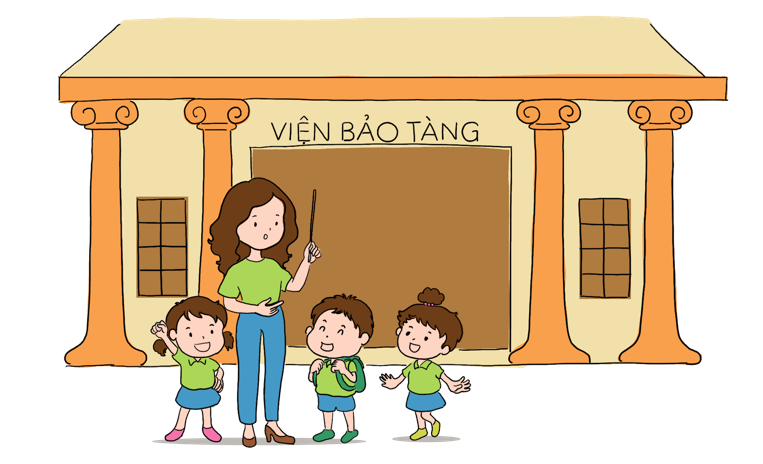
\includegraphics[width=0.8\linewidth]{Pi5_bai6}
	%		%		\vspace*{-5pt}
	%	\end{figure}
%\end{multicols}
%\newpage
%\begingroup
%\AddToShipoutPicture*{\put(110,645){
\includegraphics[scale=1]{../tieude2.pdf}}} 
%\centering
%\endgroup
%\vspace*{55pt}
%
%\begin{multicols}{2}
%	$\pmb{1.}$ Một bác nông dân chở một xe ô tô quất cảnh ra chợ Tết để bán. Sau khi bán hết cây quất cuối cùng với giá $230$ nghìn đồng, bác tính nhẩm lại thấy mình đã bán số cây quất với giá trung bình là $245$ nghìn đồng/cây. Nhưng ngay lúc ấy người mua cây quất cuối quay trở lại và chỉ cho bác thấy cành quất bị rụng quá nhiều lá, nên ông ta chỉ đồng ý mua với giá $158$ nghìn đồng. 
%	Bác chấp thuận và bán cây quất đó. Khi nhẩm tính lại, bác nông dân thấy giá trung bình của xe quất bây giờ là $242$ nghìn đồng/cây. Hỏi bác đã bán được bao nhiêu cây quất?
%	\begin{figure}[H]
	%		\centering
	%		\vspace*{-10pt}
	%		\captionsetup{labelformat= empty, justification=centering}
	%		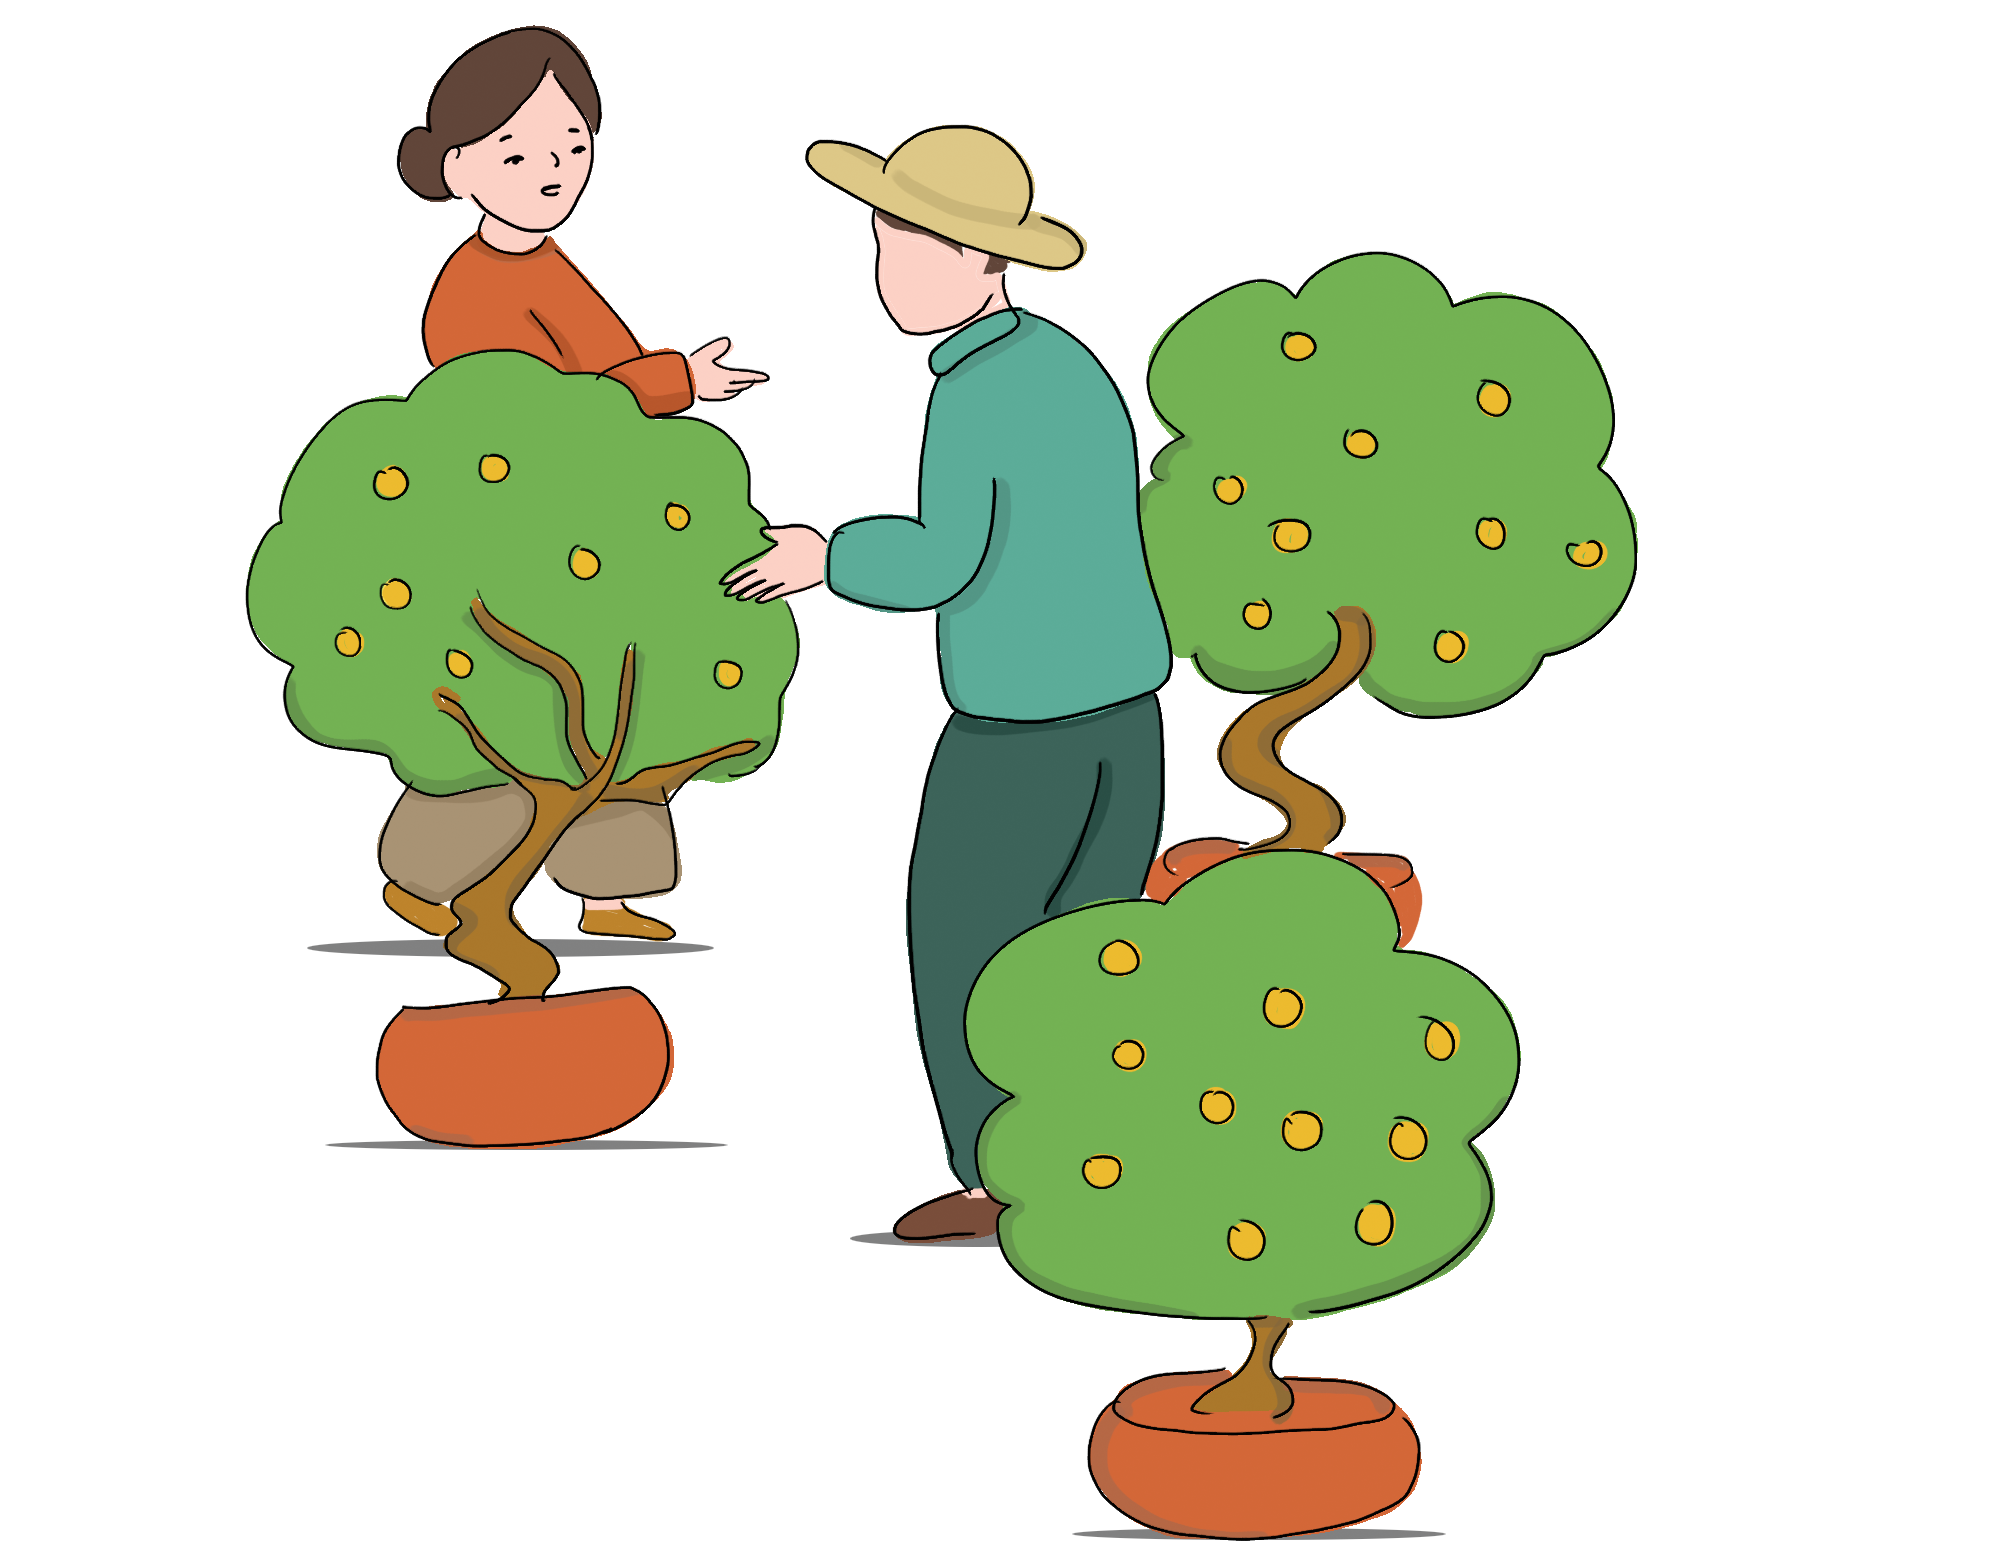
\includegraphics[width=0.7\linewidth]{Pi1_2_Bai1}
	%		\vspace*{-15pt}
	%	\end{figure}
%	\textit{Lời giải.} Gọi số cây quất là $n$, và tổng số tiền bán được của toàn bộ số quất, trừ cây cuối cùng, là $q$ (nghìn đồng). Khi đó $q+230 = 245n$ và $q+ 158 = 242n$. Trừ hai đẳng thức này ta có $72 = 3n$. Suy ra bác nông dân đã bán được $24$ cây quất.
%	\vskip 0.1cm
%	$\pmb{2.}$ Chuyện kể rằng có một người khi gặp nhà triết học và toán học Hy Lạp Pythagoras đã hỏi ông: ``Bây giờ là mấy giờ?" Pythagoras đã trả lời ``Cho đến hết ngày, còn lại hai lần của hai phần năm khoảng thời gian đã trôi qua từ lúc bắt đầu ngày". Nghe vậy, người đó chịu không thể nghĩ ra ngay được lúc họ gặp nhau là mấy giờ. Em có thể giúp trả lời lúc đó là mấy giờ được không?
%	\vskip 0.1cm
%	\textit{Lời giải.} 	Gọi $x$ là thời gian (tính theo giờ) đã trôi qua từ lúc bắt đầu ngày. Khi đó ta có hệ thức sau theo câu trả lời của Pythagoras: $24 - x = 4/5 x$. Suy ra $x = 40/3$ (giờ), có nghĩa là $13$ giờ $20$ phút. Vậy người đó đã gặp Pythagoras lúc $13$ giờ $20$ phút.
%	\begin{figure}[H]
	%		\centering
	%		\vspace*{-10pt}
	%		\captionsetup{labelformat= empty, justification=centering}
	%		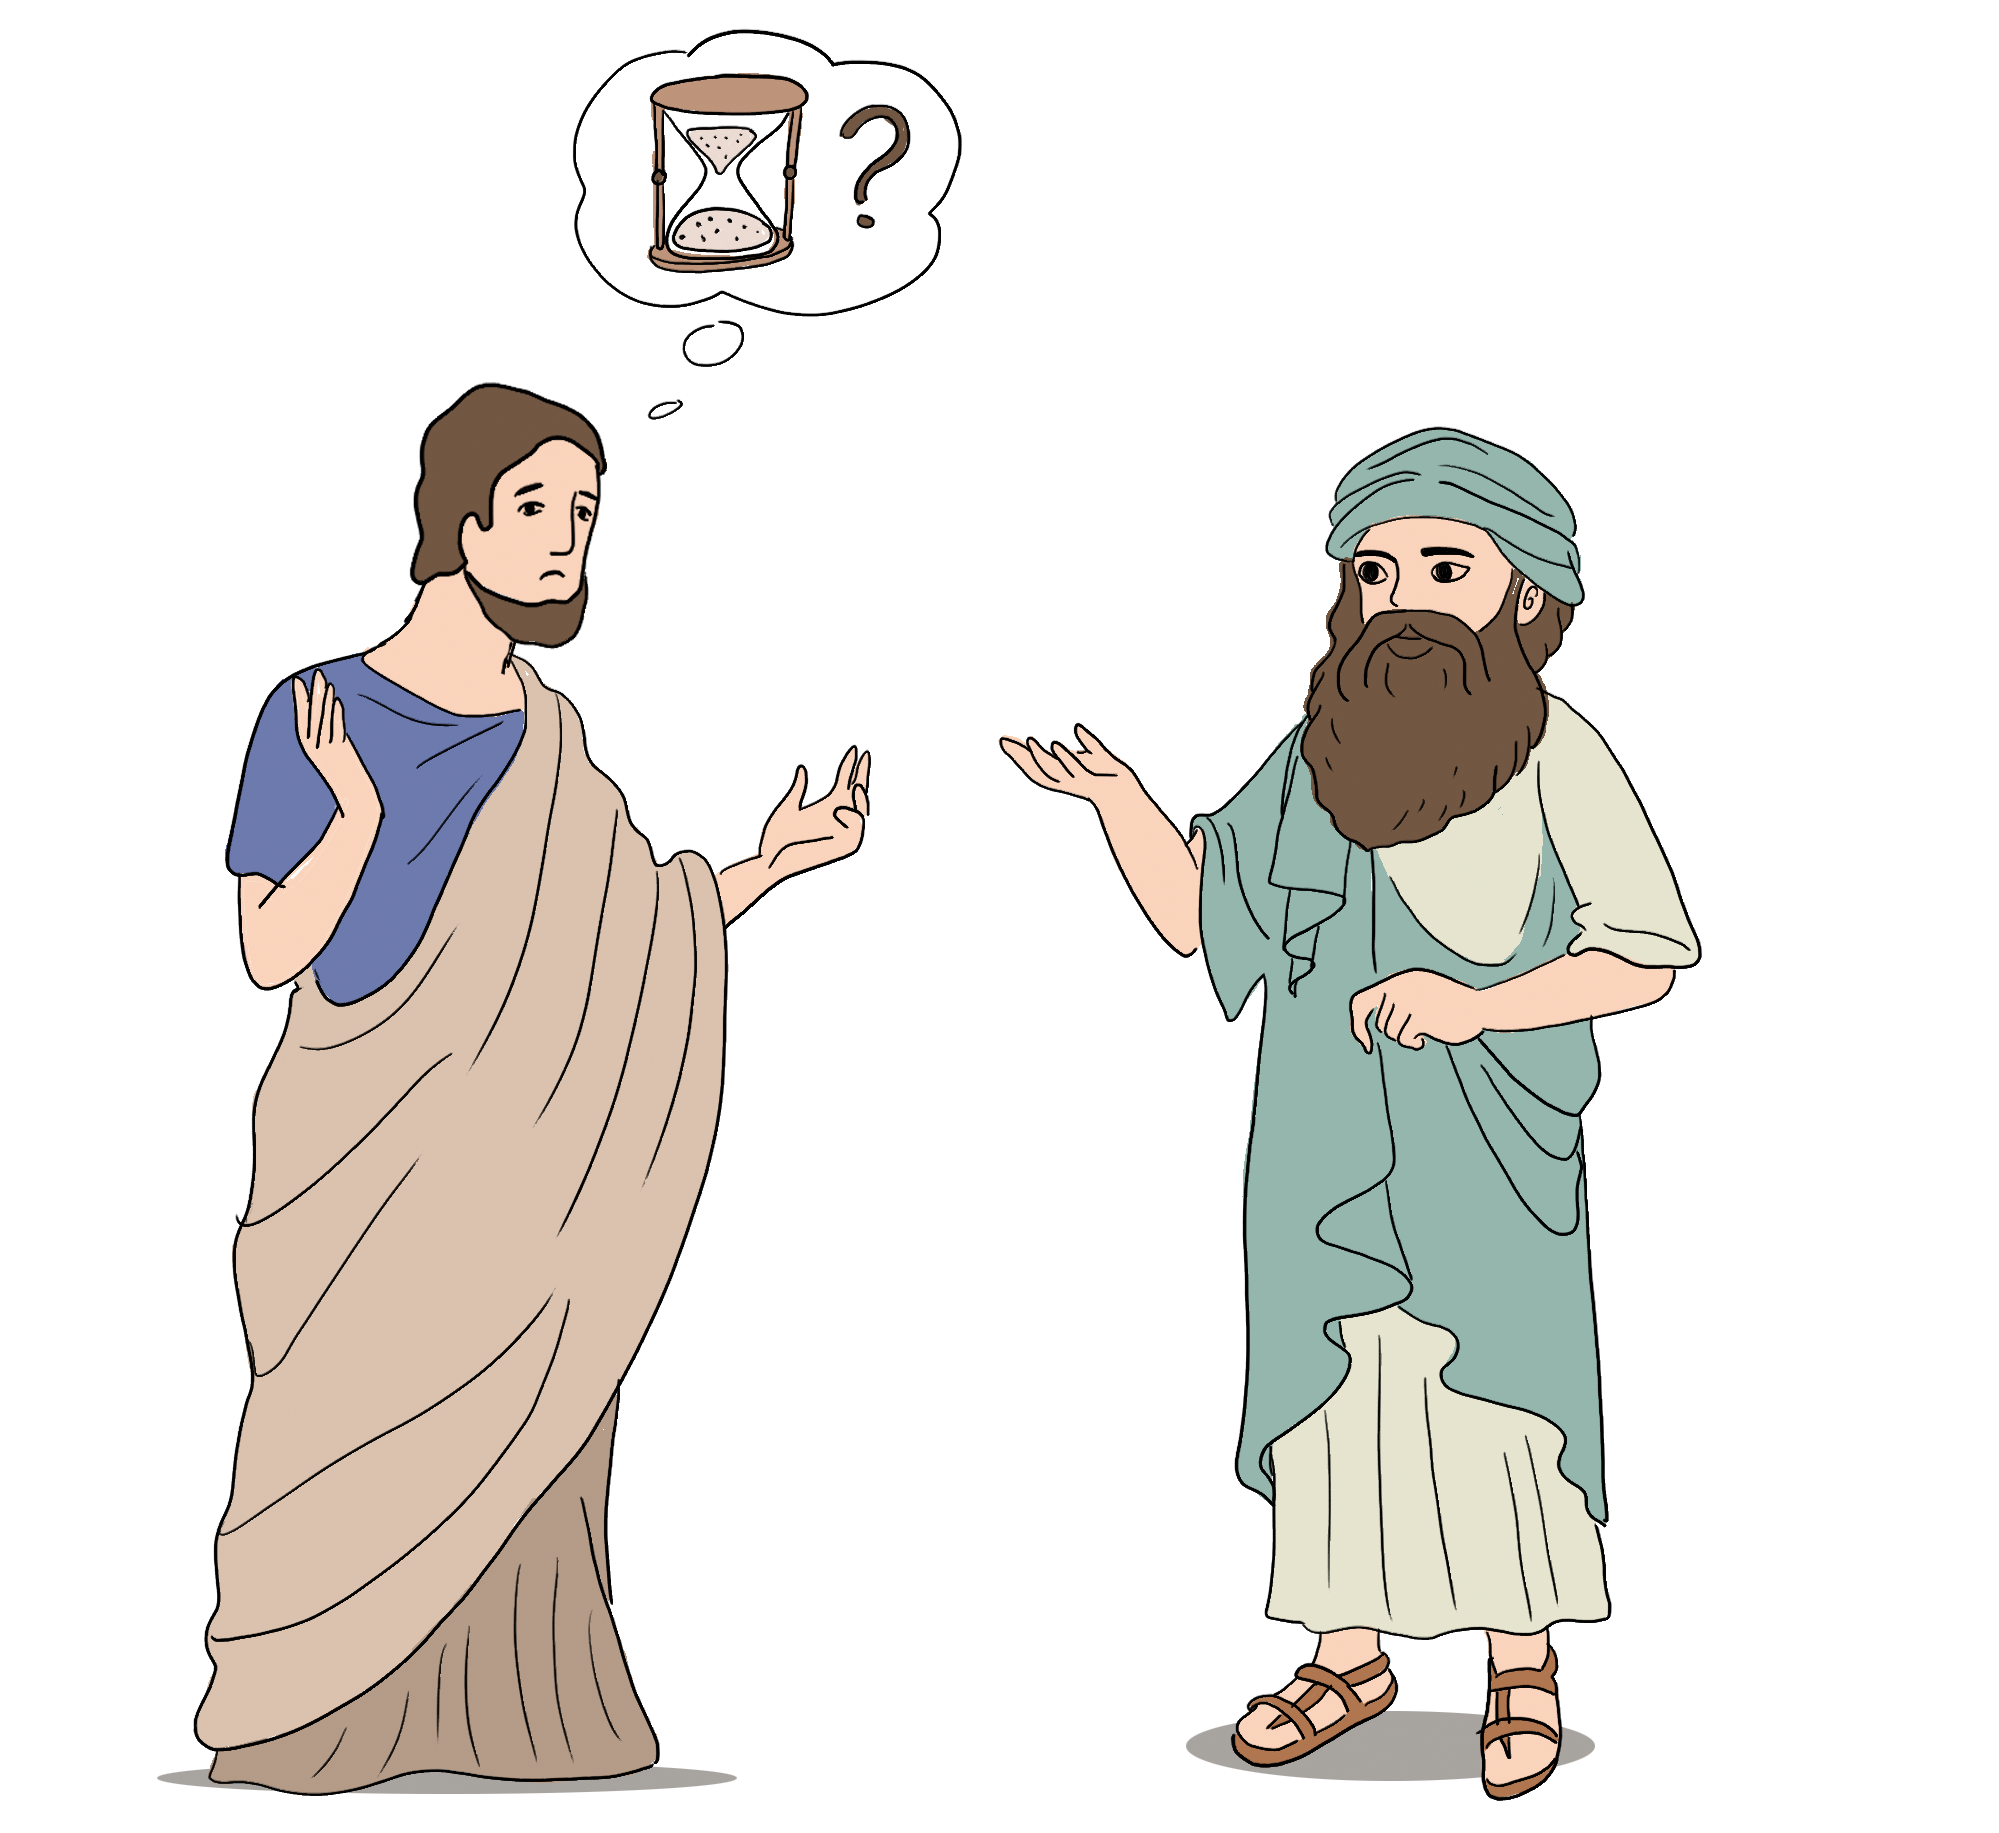
\includegraphics[width=0.6\linewidth]{Pi1_2_Bai2}
	%		\vspace*{-10pt}
	%	\end{figure}
%	$\pmb{3.}$ Một tháng trước bà Hoa ra chợ mua một cân khoai tây, một cân thịt và một chục trứng. Chủ nhật vừa rồi, khoai tây tăng lên gấp $3$, thịt gấp $4$ lần còn trứng đắt gấp $5$ lần, nên bà Hoa phải trả $600$ nghìn cho từng ấy món hàng như lần thứ nhất. Hôm nay thì khoai lại đắt gấp $6$ lần so với tháng trước, thịt đắt gấp $5$ lần còn trứng chỉ đắt gấp $4$ lần nên bà Hoa lại phải trả $660$ nghìn với cùng một lượng hàng. Hỏi bà Hoa đã trả bao nhiêu tiền cho lần mua thứ nhất?
%	\begin{figure}[H]
	%		\centering
	%		\vspace*{-10pt}
	%		\captionsetup{labelformat= empty, justification=centering}
	%		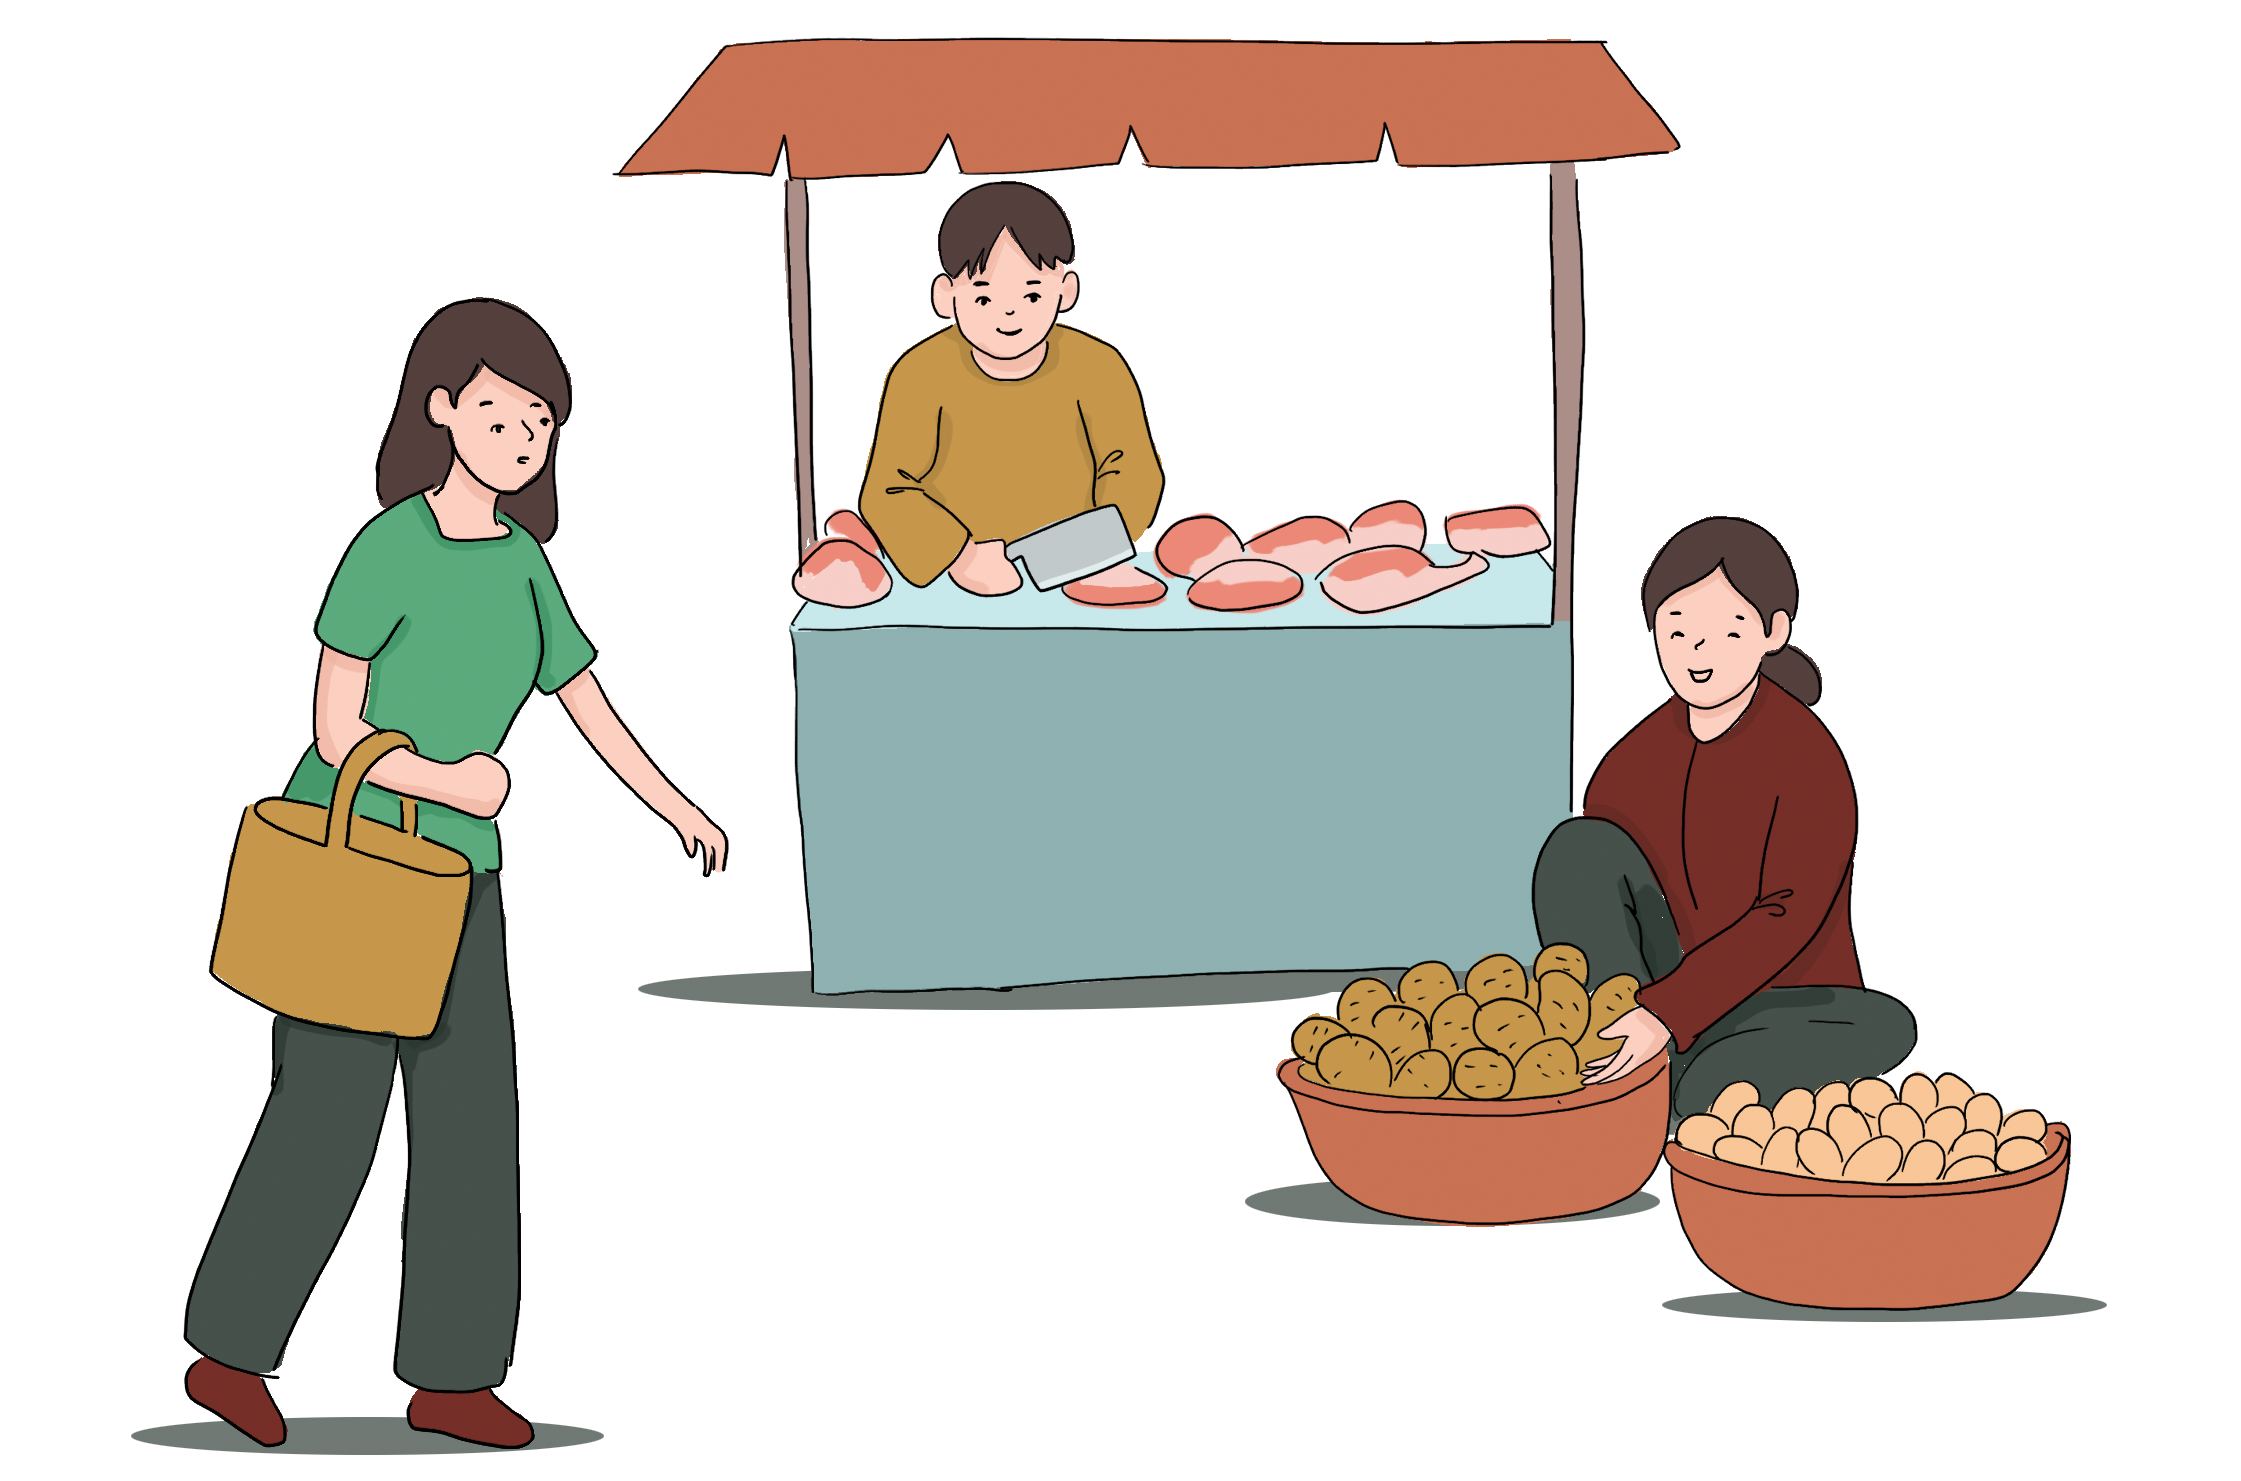
\includegraphics[width=0.6\linewidth]{Pi1_2_Bai3}
	%		\vspace*{-10pt}
	%	\end{figure}
%	\textit{Lời giải.} 	Giả sử vào tháng trước trong lần mua đầu tiên giá một cân khoai tây là $a$ (nghìn đồng), giá một cân thịt là $b$ (nghìn đồng) và giá một chục trứng là $c$ (nghìn đồng). Khi đó trong lần mua thứ nhất bà Hoa đã trả $a + b + c$ (nghìn), trong lần mua thứ hai là $3a+4b+5c = 600$ và trong lần mua thứ ba là $6a + 5b+ 4c = 660$. Cộng hai đẳng thức cuối này, ta có $9(a+b+c)= 1260$. Suy ra $a+b+c = 140$. Vậy vào tháng trước bà Hoa chỉ phải trả có $140$ nghìn đồng.
%	\vskip 0.1cm
%	$\pmb{4.}$ Trong một buổi dạ hội nọ mỗi quý ông đã hân hạnh khiêu vũ với ba quý bà, còn mỗi quý bà cũng đã khiêu vũ với ba quý ông. Em hãy chỉ ra rằng số quý ông và số quý bà tham gia dạ hội là bằng nhau.
%	\begin{figure}[H]
	%		\centering
	%		\vspace*{-5pt}
	%		\captionsetup{labelformat= empty, justification=centering}
	%		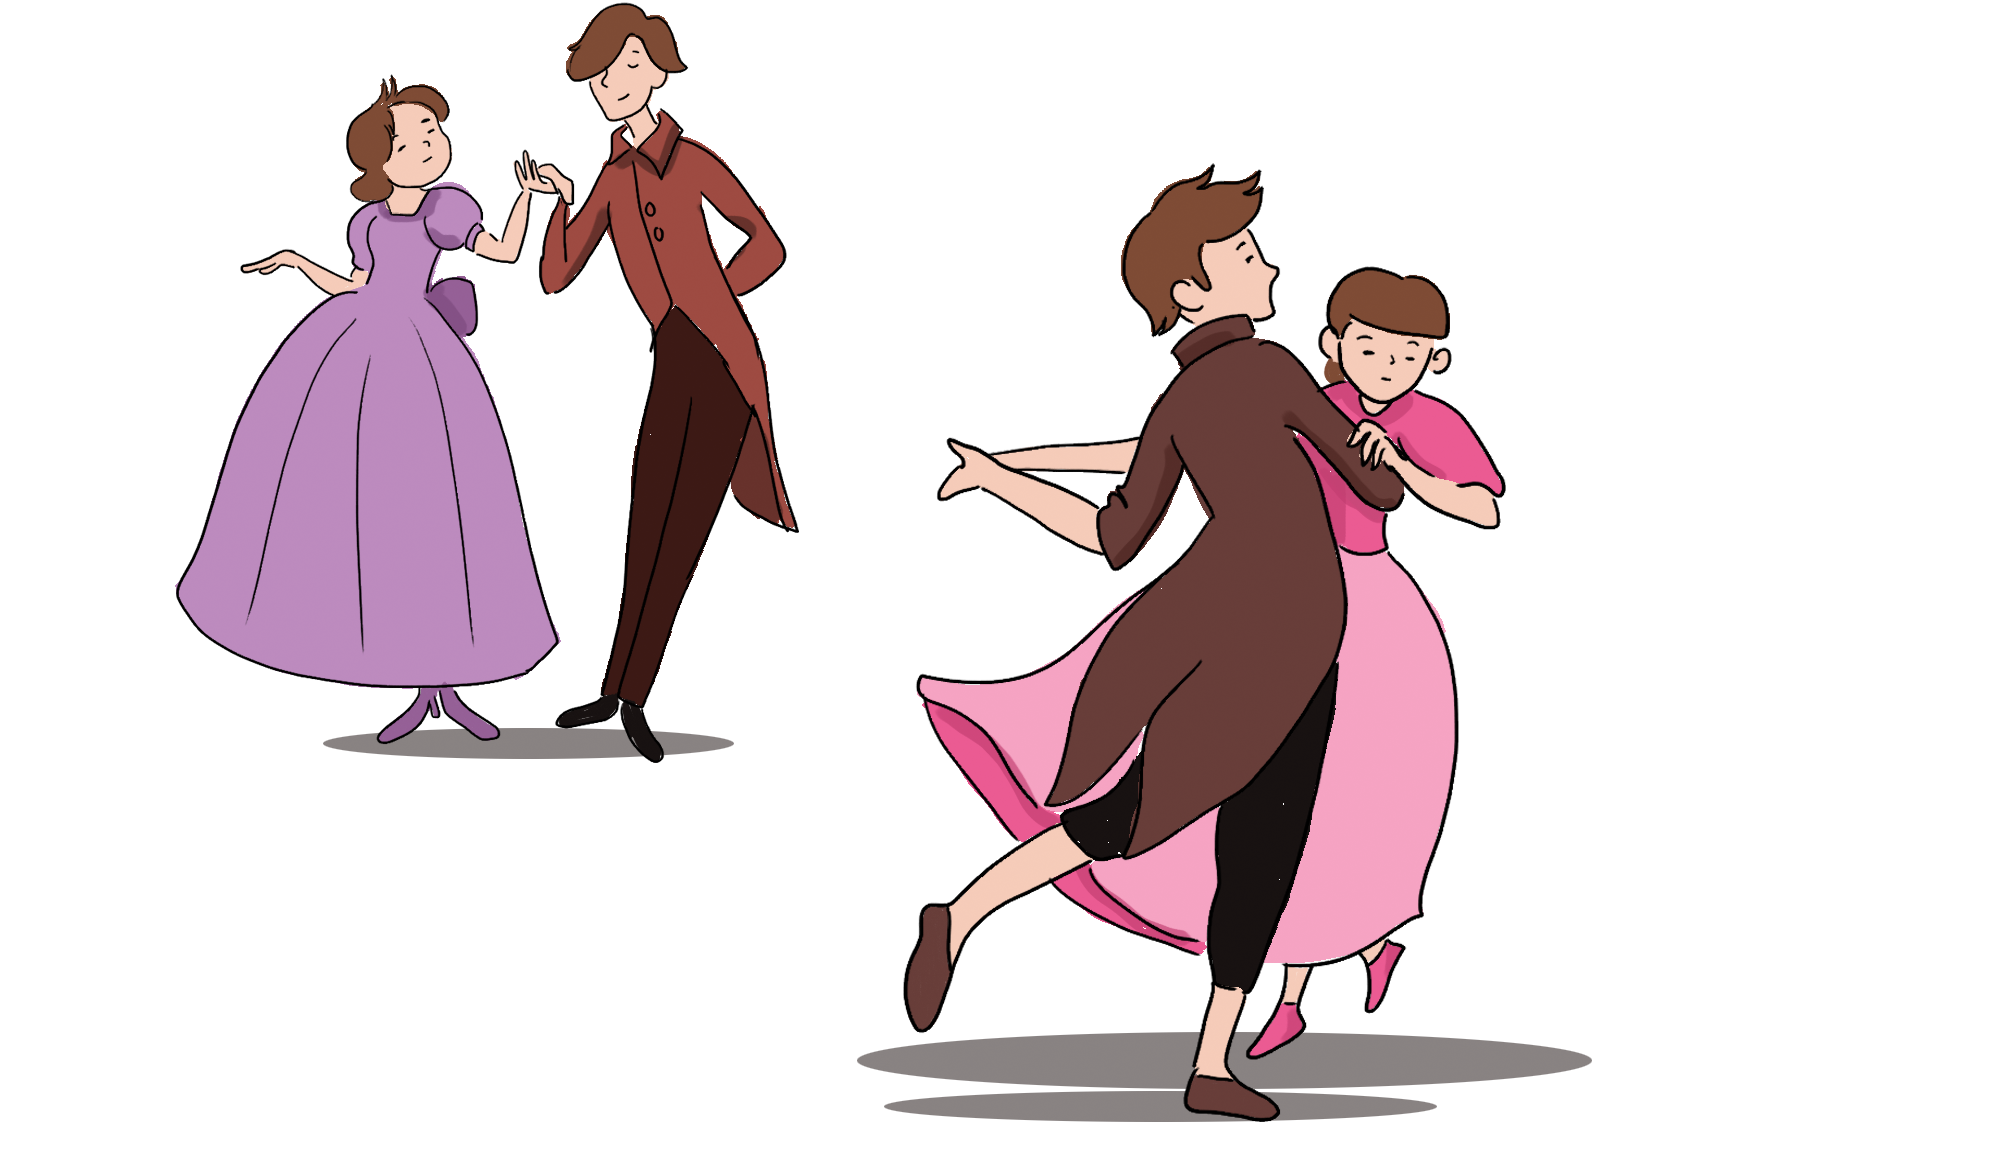
\includegraphics[width=0.75\linewidth]{Pi1_2_Bai4}
	%		\vspace*{-10pt}
	%	\end{figure}
%	\textit{Lời giải.} Ta sẽ tính tổng tất cả các cặp đã khiêu vũ với nhau. Một mặt, tổng này sẽ bằng $3$ lần số các quý ông, mặt khác nó lại bằng $3$ lần số các quý bà. Vì thế số các quý ông bằng số các quý bà.
%	\vskip 0.1cm
%	$\pmb{5.}$ 	Sau khi kết thúc một giải thi cờ vua, ban tổ chức nhận thấy mỗi kỳ thủ tham gia đã có số trận thắng khi chơi bằng quân trắng bằng đúng tổng số trận thắng của toàn bộ các kỳ thủ còn lại khi chơi quân đen. Em hãy chỉ ra rằng tất cả các kỳ thủ tham gia thi đấu đã có số trận thắng là như nhau.
%	\begin{figure}[H]
	%		\centering
	%		\vspace*{-5pt}
	%		\captionsetup{labelformat= empty, justification=centering}
	%		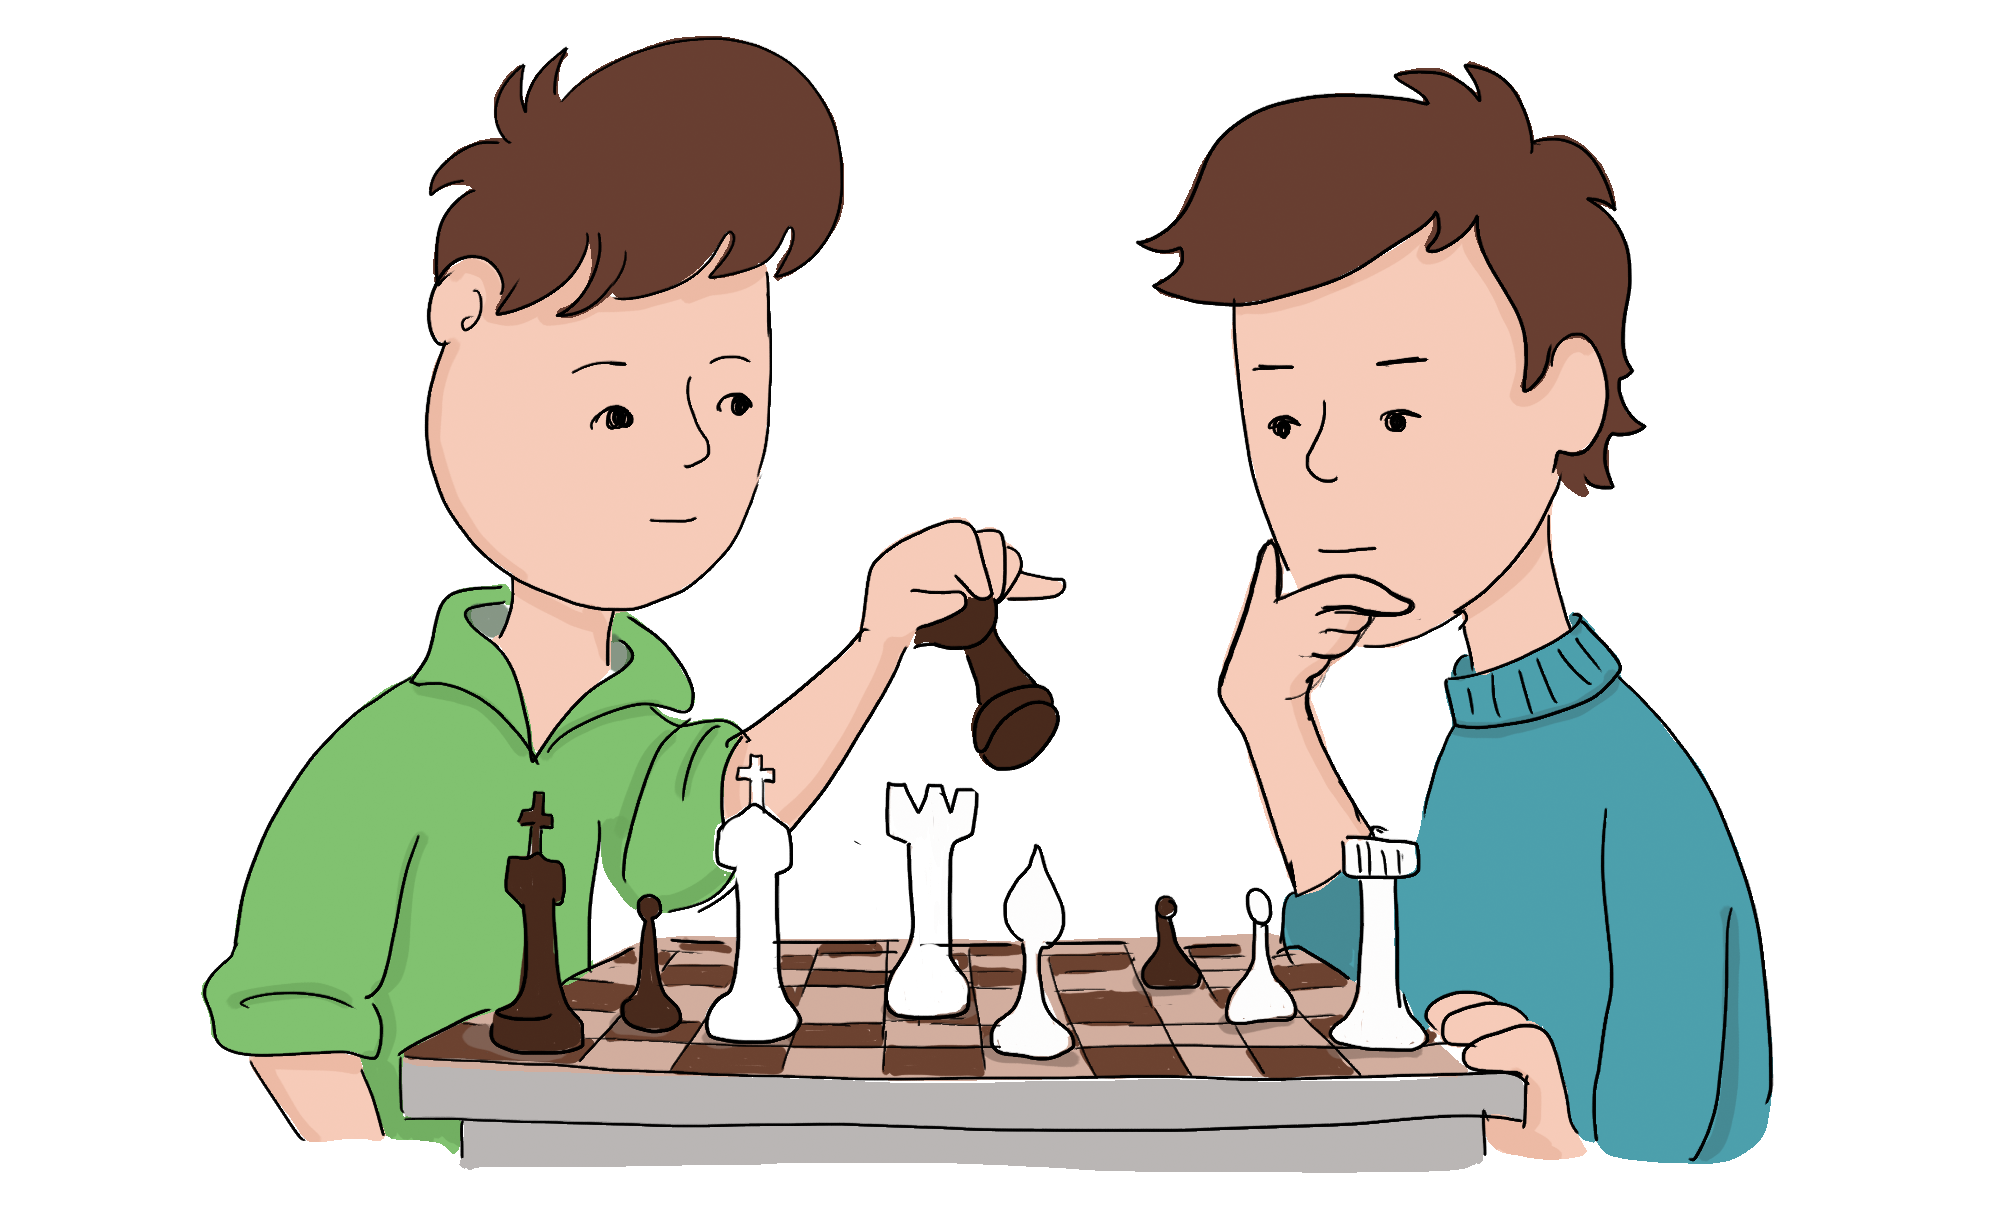
\includegraphics[width=0.6\linewidth]{Pi1_2_Bai5}
	%		\vspace*{-10pt}
	%	\end{figure}
%	\textit{Lời giải.} Các em có thể nhận thấy số trận thắng của mỗi kỳ thủ tham gia giải bằng đúng tổng số trận thắng của tất cả các kỳ thủ (kể cả chính kỳ thủ đó) khi chơi bằng quân đen. Vì thế mọi kỳ thủ tham gia đã có số trận thắng bằng nhau.
%	\vskip 0.1cm
%	$\pmb{6.}$ Vào một ngày Chủ nhật nọ, Vinh và người em trai nhỏ tuổi hơn là Minh  đạp hai chiếc xe tới hiệu sách trung tâm cách nhà vài cây số. Tại đó mỗi người chọn mua một cuốn sách quý mà nhóm bạn bè cũ đang bàn luận khen ngợi thường xuyên mấy năm nay trên Facebook. Mỗi người đều lấy tổng tất cả các chữ số của tất cả các trang sách mình đã mua và nhận thấy rằng số đó bẳng năm sinh của mình. Vậy ai  trong số hai anh em Vinh và Minh  đang đi học lớp  bồi dưỡng Toán cho học sinh phổ thông nhỉ?
%	\begin{figure}[H]
	%		\centering
	%		\vspace*{-5pt}
	%		\captionsetup{labelformat= empty, justification=centering}
	%		
\includegraphics[width=0.8\linewidth]{Pi1_2_Bai6}
	%		\vspace*{-10pt}
	%	\end{figure}
%	\textit{Lời giải.} 	Trước tiên ta tính tổng chữ số của tất cả các số từ $1$ tới $99$. Nhận thấy rằng mỗi chữ số, trừ chữ số $0$ đều xuất hiện $10$ lần ở hàng chục, và cũng $10$ lần ở hàng đơn vị, nghĩa là $20$ lần tổng cộng. Do $1+2+ \cdots+9=45$, nên tổng này bằng  $900$. Tổng các chữ số của các số từ $100$ tới $199$ sẽ lớn hơn tổng trước là $100$. Vì thế tổng các chữ số của các số từ $1$ tới $199$ bằng $1900$. Vì vậy ta xét một vài trường hợp sau.
%	\begin{table}[H]
	%		\centering
	%		\vspace*{-5pt}
	%		\captionsetup{labelformat= empty, justification=centering}
	%		\renewcommand{\arraystretch}{1.05}
	%		\begin{tabular}{|l|l|}
		%			\hline
		%			\textbf{Số trang sách}&	\textbf{Tổng các chữ số}\\
		%			\hline
		%			$200$&	$1900+2 =1902$\\
		%			\hline
		%			$202$&	$1902+3+4=1909$\\
		%			\hline
		%			$204$&	$1909+5+6=1920$\\
		%			\hline
		%			$206$&	$1920+7+8=1935$\\
		%			\hline
		%			$208$&	$1935+9+10=1954$\\
		%			\hline
		%			$210$&	$1954+11+3=1968$\\
		%			\hline
		%			$212$&	$1968+4+5=1977$\\
		%			\hline
		%			$214$&	$1977+6+7=1990$\\
		%			\hline
		%			$216$&	$1990+8+9=2007$\\
		%			\hline
		%			$217$&	$2007+10=2017$\\
		%			\hline
		%			$218$&	$2017+11=2028$\\
		%			\hline
		%		\end{tabular}
	%		\vspace*{-5pt}
	%	\end{table}
%	Các em thấy ngay chỉ có người sinh năm $2007$ trong số hai anh em mới có thể là học sinh phổ thông. Người đó cũng không thể là anh, vì nếu vậy người em trai sinh năm $2017$ đến giờ mới có $5$ tuổi không thể tự đi xe đạp vài cây số để mua sách dày hơn hai trăm trang và về nhà tự làm tính cộng hết từng đó chữ số, hơn nữa lại có nhóm bạn bè cũ trên Facebook bàn luận về cuốn sách tới mấy năm rồi. Vì vậy các em kết luận được người sinh năm $2007$ là em và có tên là Minh.
%\end{multicols}
%\newpage
%\begingroup
%\thispagestyle{toancuabinone}
%%\blfootnote{$^1$\color{toancuabi}Ottawa, Canada.}
%\AddToShipoutPicture*{\put(60,733){
\includegraphics[width=17.2cm]{../mathc.pdf}}}
%%\AddToShipoutPicture*{\put(-2,733){
\includegraphics[width=17.2cm]{../mathl.pdf}}} 
%\AddToShipoutPicture*{\put(136,648){
\includegraphics[scale=1]{../tieude12.pdf}}} 
%\centering
%\endgroup
%\graphicspath{{../toancuabi/pic/}}
%\vspace*{55pt}
%
%\begin{multicols}{2}
%	It is a beautiful and blossoming Spring day. Tom and Ken are visiting the National Zoo in Washington, D.C. 
%	\vskip 0.1cm
%	As they eagerly walk through the entrance, Tom says: ``The National Zoo is currently home to about $2{,}100$ animals; they comprise hundreds of species. In the zoo, the species need an environment that resembles their natural habitat as closely as possible. The animals must be accommodated to a lifestyle similar to their wild counterparts."
%	\vskip 0.1cm
%	``Oh I see. If they climb, they get trees or rocks. If they swim, they are in ponds, lakes and rivers. If they like to burrow, they own caves and tunnels. If they fly, they already have the sky." Ken replies excitedly.
%	\vskip 0.1cm
%	``Beautiful! The terrains are designed to make the animals feel secure as well. Some animals are tamed: giraffes like visitors watching and feeding them. Some animals don't like to see the crowd. These hermitian animals like leopards need a jungle where they can retreat from humans. In order to protect those creatures and conserve wildlife, zoologists must study Nature very well." Tom continues.
%	\vskip 0.1cm
%	``From the brochure, we can learn valuable scientific information and classifications. Can you tell which creatures are sociable and which animals are solitary?" Tom asks.
%	\vskip 0.1cm
%	``Well, let's see." Ken takes out the brochure. He reads out loud:
%	\vskip 0.1cm
%	--	Sociable: squirrels, primates, and so on.
%	\vskip 0.1cm
%	--	Solitary: leopards, giant pandas, and so on. 
%	\vskip 0.1cm
%	Tom nods: ``Wonderful! To express and see better, you can draw a circle like this. Put those solitary inside the circle and those sociable outside of the circle. This is called a \textit{Venn diagram}."
%	\begin{figure}[H]
%			\vspace*{-10pt}
%			\centering
%			\captionsetup{labelformat= empty, justification=centering}
%			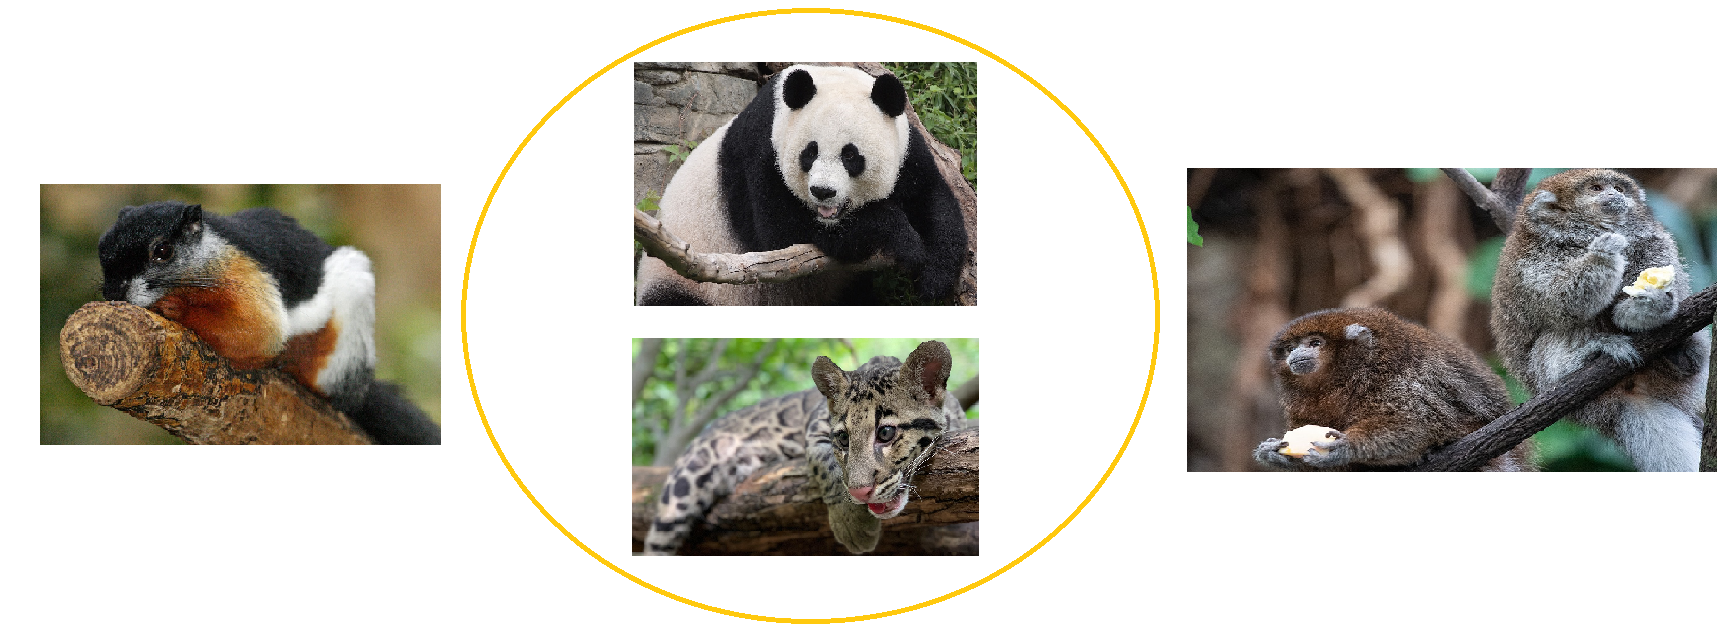
\includegraphics[width= 1\linewidth]{p1}
%			\vspace*{-15pt}
%		\end{figure}	
%	Tom continues: ``In math, we call this circle a set: the `solitary' set consisting of solitary species. The hermitian creatures inside the circle are called \textit{elements} of the `solitary' set. The tamed and sociable animals outside of the circle are not elements of the `solitary' set."
%	\vskip 0.1cm
%	Ken listens attentively: ``That's cool. So if I want to classify animals by their habitats, I can draw a Venn diagram of $3$ circles. One for landscapes, one for water, and one for the sky. The mammals live on land. The fish swim in water. The birds fly high." Ken replies.
%	\vskip 0.1cm
%	Tom slows down to emphasize: ``Perfect! And you have $3$ sets: the set of `on--land' animals, the set of `aquatic' animals, and the set of `on--sky' animals. Does it make sense?"
%	\vskip 0.1cm
%	``It is as clear as day." Ken answers, full of smiles.
%	\vskip 0.1cm
%	As they move on, Tom says: ``And here are some fun facts. Amphibians, like turtles and frogs, live both on grasslands and in the lakes. So they belong to both the on--land set and the aquatic set. You can draw to express the overlap." 
%	\vskip 0.1cm
%	``Really? There are creatures that can live in both environments!" Ken is surprised.
%	\vskip 0.1cm
%	Tom gives another example: ``Not just that! The bald eagles symbolize the national bird of the Americans. They hunt for fishes near the water surface and also hunt over grasslands. They belong to both ecosystems: the sky and the land."
%	\begin{figure}[H]
%			\vspace*{-10pt}
%			\centering
%			\captionsetup{labelformat= empty, justification=centering}
%			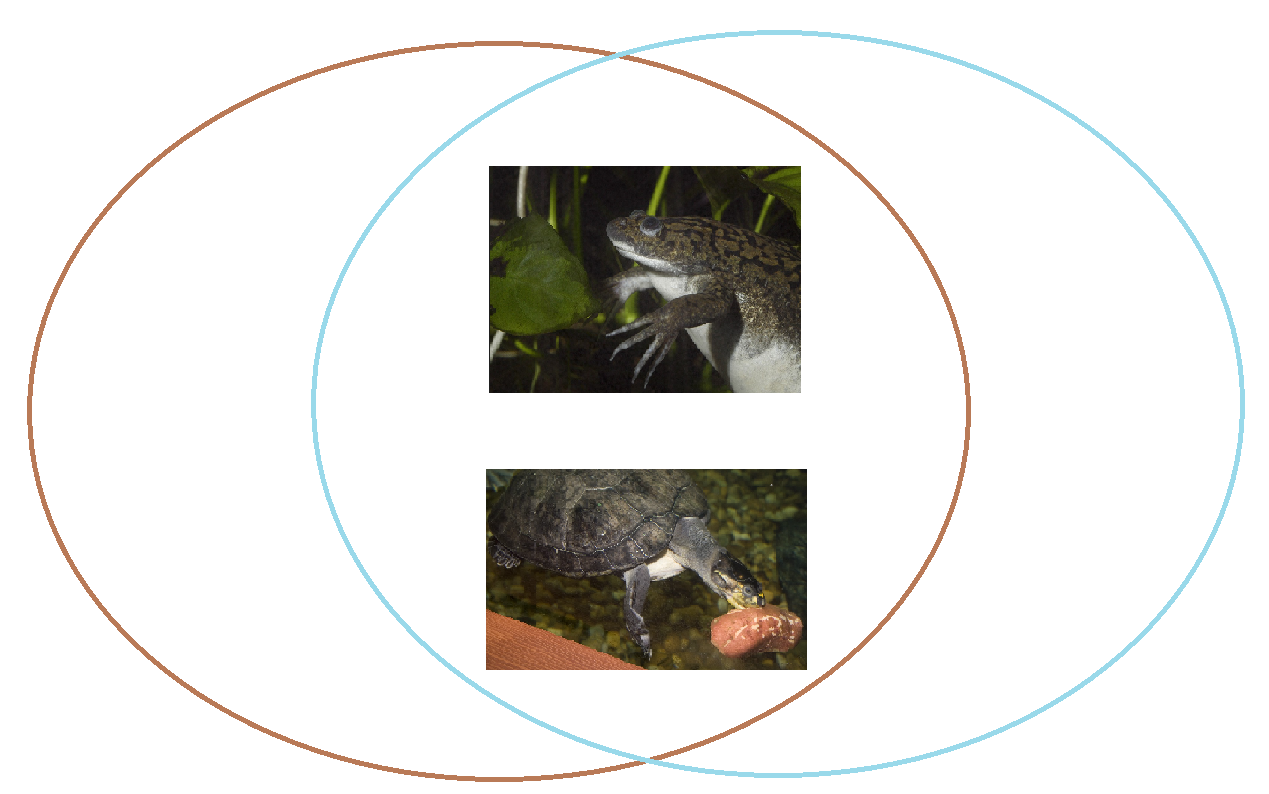
\includegraphics[height= 0.3\linewidth]{p2}
%			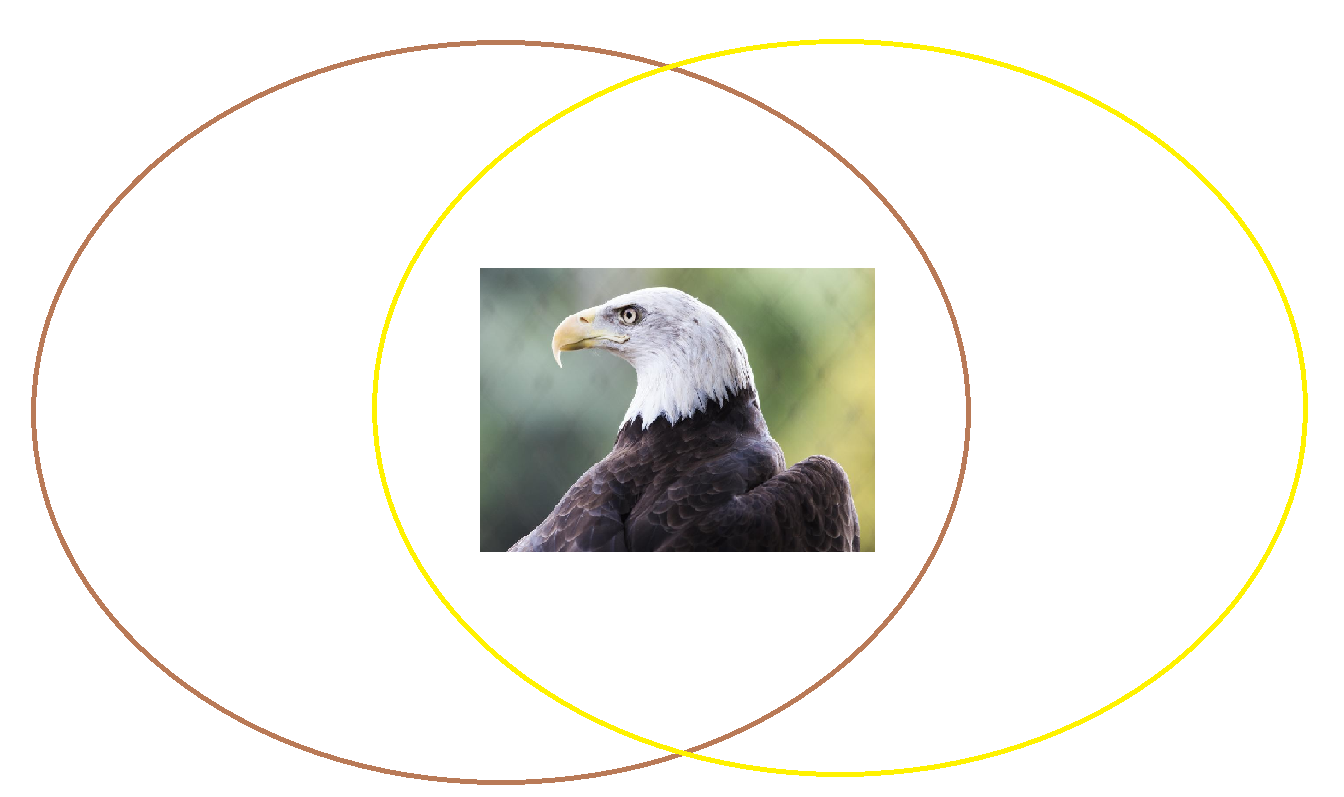
\includegraphics[height= 0.3\linewidth]{p3}
%			\vspace*{-25pt}
%		\end{figure}
%	Tom continues: ``Those overlapping areas are called \textit{intersections} of two sets. If you take all animals in two circles, the sky and the land say, you have a much bigger set of animals. You are thinking of all animals inhabiting either landscapes or the sky. Math lovers call it the \textit{union} of two sets." 
%	\vskip 0.1cm
%	Tom tries to conclude: ``Red--crowned cranes are found in Russia, China, Mongolia and Japan. In Japan, they forage regularly on pasturelands. They are also aquatic: they feed and nest in rivers or marshes with relatively deep water. They can fly well and migrate in flocks. These cranes inhabit all $3$ ecosystems: land, water and sky." 
%	\begin{figure}[H]
%			\vspace*{-5pt}
%			\centering
%			\captionsetup{labelformat= empty, justification=centering}
%			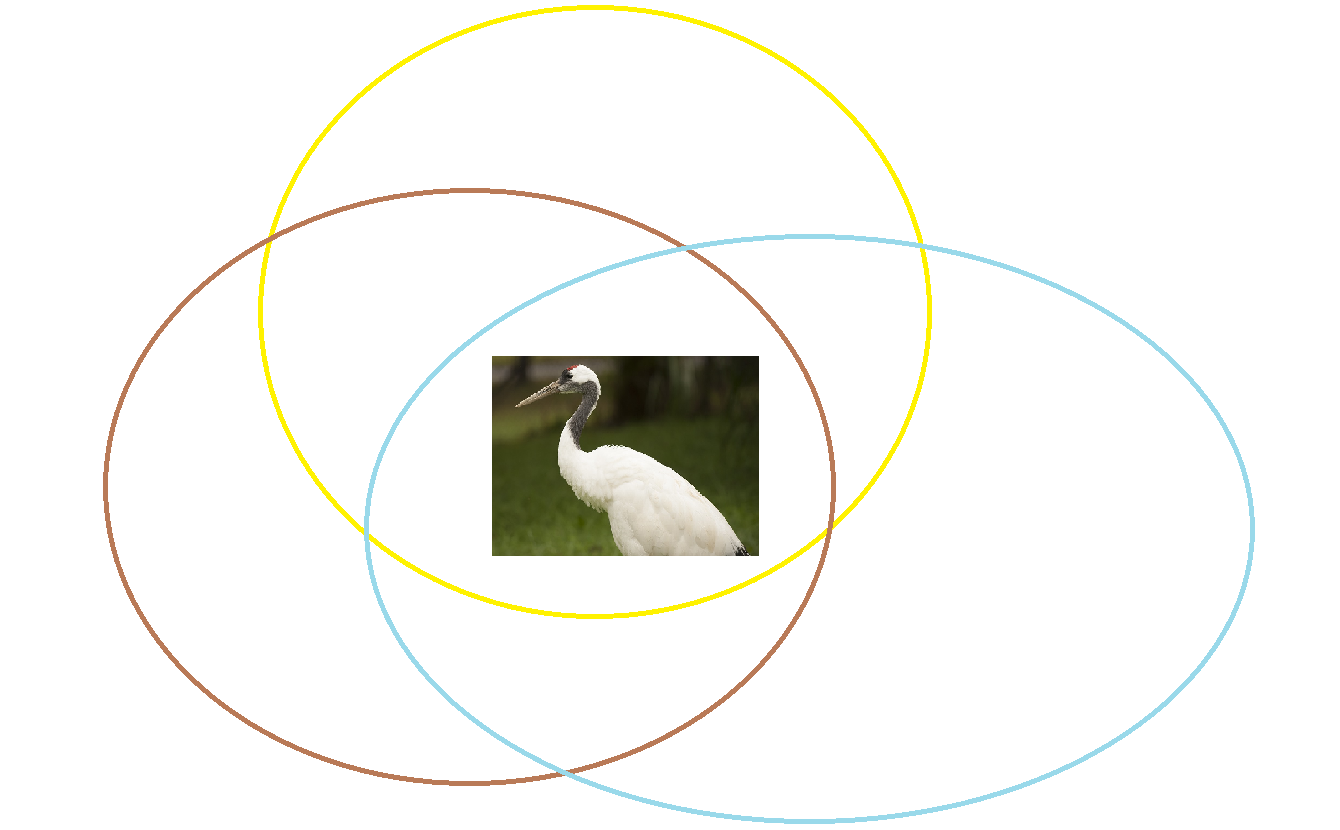
\includegraphics[width= 0.7\linewidth]{p4}
%			\vspace*{-10pt}
%		\end{figure}
%	Tom: ``In the large, the union of these $3$ sets is called the \textit{total set}."
%	\vskip 0.1cm
%	Ken's voice is filled with happiness: ``That is our beloved Earth!"
%	\vskip 0.1cm
%	Tom: ``Voilà!"
%	\vskip 0.1cm
%	Ken: ``Can we start with the Asia Trail? I can't wait to see the cute giant pandas!"
%	\vskip 0.1cm
%	``Ok, let's go!"
%	\vskip 0.1cm
%	The above article is meant to be an introduction to Venn diagram for children in early Grades (such as Grades $1$, $2$ and $3$) who have not met this concept before.
%	\vskip 0.1cm
%	Photo source: \url{https://nationalzoo.si.edu/}
%	\vskip 0.1cm
%	\PIbox{
%			{\centerline{\textbf{\color{toancuabi}Vocabulary}}}
%			\vskip 0.1cm
%			\textbf{\color{toancuabi}Natural sciences}
%			\vskip 0.1cm
%			{\color{toancuabi}species:} (n) giống loài
%			\vskip 0.1cm
%			{\color{toancuabi}habitat:} (n)  môi trường sống
%			\vskip 0.1cm
%			{\color{toancuabi}ecosystem:} (n)  hệ sinh thái
%			\vskip 0.1cm
%			{\color{toancuabi}symbolize:} (v)  biểu tượng
%			\vskip 0.1cm
%			{\color{toancuabi}burrow:} (v)  đào hang
%			\vskip 0.1cm
%			{\color{toancuabi}terrain:} (n)  địa hình
%			\vskip 0.1cm
%			{\color{toancuabi}solitary:} (adj)  đơn độc
%			\vskip 0.1cm
%			{\color{toancuabi}sociable:} (adj)  bầy đàn
%			\vskip 0.1cm
%			{\color{toancuabi}aquatic:} (adj)  dưới nước
%			\vskip 0.1cm
%			{\color{toancuabi}grassland:} (n)  đồng cỏ
%			\vskip 0.1cm
%			{\color{toancuabi}pastureland:} (n)  thảo nguyên
%			\vskip 0.1cm
%			{\color{toancuabi}feed:} (v)  nuôi, kiếm ăn
%			\vskip 0.1cm
%			{\color{toancuabi}hunt:} (v)  săn mồi 
%			\vskip 0.1cm
%			{\color{toancuabi}inhabit:} (v)  sinh sống 
%			\vskip 0.1cm
%			{\color{toancuabi}nest:} (v)  làm tổ 
%			\vskip 0.1cm
%			{\color{toancuabi}migrate:} (v)  di cư
%			\vskip 0.1cm
%			{\color{toancuabi}flock:} (n)  đàn, bầy
%			\vskip 0.1cm
%			{\color{toancuabi}amphibian:} (n)  động vật lưỡng cư
%			\vskip 0.1cm
%			{\color{toancuabi}crane:} (n)  con hạc / con sếu
%			\vskip 0.1cm
%			{\color{toancuabi}eagle:} (n)  đại bàng
%			\vskip 0.1cm
%			{\color{toancuabi}frog:} (n)  con ếch
%			\vskip 0.1cm
%			{\color{toancuabi}leopard:} (n)  con báo
%			\vskip 0.1cm
%			{\color{toancuabi}monkey:} (n)  con khỉ
%			\vskip 0.1cm
%			{\color{toancuabi}panda:} (n)  gấu trúc
%			\vskip 0.1cm
%			{\color{toancuabi}squirrel:} (n)  con sóc
%			\vskip 0.1cm
%			{\color{toancuabi}turtle:} (n)  con rùa 
%			\vskip 0.1cm
%			\textbf{\color{toancuabi}Mathematics}
%			\vskip 0.1cm
%			{\color{toancuabi}Venn diagram:} (n)  sơ đồ Venn / biểu đồ Venn
%			\vskip 0.1cm
%			{\color{toancuabi}set:} (n)  tập hợp
%			\vskip 0.1cm
%			{\color{toancuabi}intersection of $2$ sets:} (n)  giao của $2$ tập hợp
%			\vskip 0.1cm
%			{\color{toancuabi}union of $2$ sets:} (n)  hợp của $2$ tập hợp
%			\vskip 0.1cm
%			{\color{toancuabi}total set:} (n)  tập hợp tổng
%			\vskip 0.1cm
%			{\color{toancuabi}concept:} (n)  khái niệm}
%\end{multicols}
%\newpage
%\begingroup
%\thispagestyle{toancuabinone}
%\blfootnote{$^1$\color{toancuabi}Ottawa, Canada.}
%\AddToShipoutPicture*{\put(60,733){
\includegraphics[width=17.2cm]{../mathc.pdf}}}
%%\AddToShipoutPicture*{\put(-2,733){\includegraphics[width=17.2cm]{../mathl.pdf}}} 
%\AddToShipoutPicture*{\put(178,675){\includegraphics[scale=1]{../tieudea.pdf}}} 
%\centering
%\endgroup
%\graphicspath{{../toancuabi/pic/}}
%\vspace*{35pt}
%
%\begin{multicols}{2}
%	In this article, some problems of paths on boards are discussed.
%	They highlight the relations of cells in same column or row.
%	\vskip 0.2cm
%	\PIbox{{\color{toancuabi}\textbf{\color{toancuabi}Example} (Who is the taller one?)}
%			\vskip 0.1cm
%			One hundred students are positioned in $10 \times 10$ grids,
%			each of the rows and columns contains exactly $10$ students.
%			From each of the $10$ columns the \textit{shortest} student is selected,
%			and the \textit{tallest} of these $10$ students is tagged as $T$.
%			Next the \textit{tallest} student from each rows is selected,
%			and from these $10$ students the \textit{shortest} is tagged as $S$.
%			Which of the two tagged students is the taller if they are two different people?}
%	\vskip 0.2cm
%	\textit{Solution.}
%		If $S$ and $T$ are in the same column, then $T$ is among the shortests of each column,
%		so $T$ is the shortest in its own column, thus $T$ is shorter than $S$.
%		If $S$ and $T$ are in the same row, then $S$ is among the tallests of each column,
%		so it is the tallest in its own row, thus $T$ is shorter than $S$.
%		\begin{figure}[H]
%				\vspace*{-5pt}
%				\centering
%				\captionsetup{labelformat= empty, justification=centering}
%				\begin{tikzpicture}[scale=0.9, toancuabi]
%						\draw (0,0) grid (5,5);
%						\draw (1.5,1.5) node{$\color{red}S$};
%						\draw (3.5,1.5) node{$I$};
%						\draw (3.5,3.5) node{$\color{cackithi!40}T$};
%					\end{tikzpicture}
%				\vspace*{-5pt}
%			\end{figure}
%		If $S$ and $T$ are in different rows and colums,
%		then there exists $I$ at the intersection of the row of $S$ and the column of $T$.
%		By definition, $T$ is shorter than $I$ and $I$ is shorter than $S$,
%		thus $T$ is shorter than $S$.
%		\vskip 0.1cm
%		Therefore, ${S}$ is the taller one.
%		\vskip 0.2cm
%		\PIbox{{\color{toancuabi}\textbf{\color{toancuabi}Example} (How many ways to form the name?)}
%				\vskip 0.1cm
%				Thanh filled a triangle of squares with the letters of her name, as shown below.
%				She counted all the $5-$letter paths that form her name T--H--A--N--H,
%				each starts from the T letter in the middle of the bottom row,
%				then goes left, right, or up. An example is also shown in the diagram.
%				What number did she get?}
%		\vskip 0.2cm
%	\begin{figure}[H]
%			\vspace*{-5pt}
%			\centering
%			\captionsetup{labelformat= empty, justification=centering}
%			\renewcommand{\arraystretch}{1.2}
%			\begin{tabular}{ccccccccc}
%					&   &   &   & H                                                &                                                  &                                                  &   &   \\
%					&   &   & H & N                                                & H                                                &                                                  &   &   \\
%					&   & H & N & A                                                & \cellcolor{cackithi!40}N & \cellcolor{cackithi!40}H &   &   \\
%					& H & N & A & \cellcolor{cackithi!40}H& \cellcolor{cackithi!40}  A  & N                                                & H &   \\
%					H & N & A & H & \cellcolor{cackithi!40}T & H                                                & A                                                & N &  H 
%				\end{tabular} 
%			\vspace*{-10pt}
%		\end{figure}
%	\textit{Solution.}
%	Consider the \textit{``half"} triangle shown in the diagram below.
%	It is easy to see that in each path, there is two choices at each steps.
%	One example is shown in the figure, when two As can be chosen after a $H$.
%	\begin{figure}[H]
%			\vspace*{-5pt}
%			\centering
%			\captionsetup{labelformat= empty, justification=centering}
%			\renewcommand{\arraystretch}{1.2}
%			\begin{tabular}{ccccl}
%					&   &                                                  &                                                  &  H                                                 \\
%					&   &                                                  &  H                                                 &  N                                                 \\
%					&   &  H                                                 &  N                                                 &  A                                                 \\
%					&  H  &  N                                                 & \cellcolor{duongvaotoanhoc!40}  A &  H                                                 \\
%					H  &  N  & \cellcolor{duongvaotoanhoc!40}  A  & \cellcolor{cackithi!40}  H  & \cellcolor{cackithi!40}  T 
%				\end{tabular}
%		\vspace*{-10pt}
%		\end{figure}
%		Therefore there are $2^4=16$ paths for a half triangle.
%		In total there are $2\cdot 16-1=31$,
%		because the vertical path formed by all the squares in the $T$ column
%		is shared by both half triangles.
%		\vskip 0.1cm
%		Thus, the number that Thanh got is $31.$
%		\vskip 0.1cm
%		\PIbox{{\color{toancuabi}\textbf{\color{toancuabi}Example} (What would be the largest number?)}
%				\vskip 0.1cm
%				In each square of the $n \times n$, $n \ge 4$ chessboard,
%				Antoine writes a number according to the following rules:
%				\vskip 0.1cm
%				$i.$ The number in each square is one of $1,2,\ldots,n^2$.
%				\vskip 0.1cm
%				$ii.$ The two numbers, in two neighbouring squares that share the same side, differ less than $3$.
%				\vskip 0.1cm
%				$iii.$ The number $3$ is written in one of the square.
%				\vskip 0.1cm
%				What is the largest number could Antoine writes on the board?}
%		\vskip 0.2cm
%		\textit{Solution.}
%		Let $m$ be the maximal number that can be written on the board.
%		\begin{figure}[H]
%				\vspace*{-5pt}
%				\centering
%				\captionsetup{labelformat= empty, justification=centering}
%				\begin{tikzpicture}[toancuabi]
%						\filldraw[cackithi!40] (0,3) rectangle (5,4);
%						\filldraw[cackithi!40] (3,0) rectangle (4,5);
%						\draw (0,0) grid (5,5);
%						\draw (1.5,3.5) node {$3$};
%						\draw (3.5,1.5) node {$m$};
%						\draw (3.5,3.5) node {$i$};
%					\end{tikzpicture}
%				\vspace*{-10pt}
%			\end{figure}
%		In the figure above, there are atmost $n-1$ squares on the row of $3$,
%		not including the square containing $3$, 
%		from the number $3$ to the intersection $i$ with the column of $m$,
%		Similarly there are atmost $n-1$ squares on the column of $m$,
%		not including the square containing $m$, 
%		from the intersection $i$ with the column of $m$ to the number $m$.
%		Thus the difference between $m$ and $3$ can not be more than
%		$2\cdot (n-1)+ 2\cdot (n-1)=4(n-1)$.
%		\vskip 0.1cm
%		Therefore, the largest value of $m$ can be $3+4(n-1)={4n-1.}$
%		\vskip 0.2cm
%		\PIbox{{\color{toancuabi}\textbf{\color{toancuabi}Example} (Colouring the paths)}
%				\vskip 0.1cm
%				In the $4 \times 4$ grid below each cell at row $i$ and column $j$ contains the value equal to $i \times j.$
%				A \textit{path} in the grid is a sequence of squares,
%				such that consecutive squares share an edge and no square occurs twice in the sequence.
%				Furthermore, the \textit{score} of a path is the sum of the point values of all squares in the path.
%				\vskip 0.1cm
%				Determine the highest possible score of a path that begins with the bottom left corner of the grid 
%				(where the number $1$ stands) and ends with the top right corner (where the number $16$ stands.)}
%		\vskip 0.2cm
%		\begin{figure}[H]
%				\vspace*{-5pt}
%				\centering
%				\captionsetup{labelformat= empty, justification=centering}
%				\begin{tikzpicture}[toancuabi]
%						\draw (0,0) grid (4,4);
%						\draw (0.5 , 0.5) node {$1$};
%						\draw (0.5 , 1.5) node {$2$};
%						\draw (0.5 , 2.5) node {$3$};
%						\draw (0.5 , 3.5) node {$4$};
%						\draw (1.5 , 0.5) node {$2$};
%						\draw (1.5 , 1.5) node {$4$};
%						\draw (1.5 , 2.5) node {$6$};
%						\draw (1.5 , 3.5) node {$8$};
%						\draw (2.5 , 0.5) node {$3$};
%						\draw (2.5 , 1.5) node {$6$};
%						\draw (2.5 , 2.5) node {$9$};
%						\draw (2.5 , 3.5) node {$12$};
%						\draw (3.5 , 0.5) node {$4$};
%						\draw (3.5 , 1.5) node {$8$};
%						\draw (3.5 , 2.5) node {$12$};
%						\draw (3.5 , 3.5) node {$16$};
%					\end{tikzpicture}
%				\vspace*{-10pt}
%			\end{figure}
%		\textit{Solution.}
%		Let us colour the squares of the grid with a chessboard pattern of black and white,
%		starting with black in the bottom left--hand corner, as show below on the left diagram.
%		A path in the grid will alternate between black and white squares,
%		beginning and ending on black.
%		Thus, any path cannot contain all $8$ white squares.
%		\vskip 0.1cm
%		\begin{figure}[H]
%				\vspace*{-5pt}
%				\centering
%				\captionsetup{labelformat= empty, justification=centering}
%				\begin{tikzpicture}[toancuabi]
%						\foreach \y in {0,2}{
%							\foreach \x in {0,2}{
%								\fill[cackithi!40] (\x,\y) rectangle (1+\x,1+\y) rectangle (2+\x,2+\y);}}
%						\draw (0,0) grid (4,4);
%						\draw (0.5 , 0.5) node {$1$};
%						\draw (0.5 , 1.5) node {$2$};
%						\draw (0.5 , 2.5) node {$3$};
%						\draw (0.5 , 3.5) node {$4$};
%						\draw (1.5 , 0.5) node {$2$};
%						\draw (1.5 , 1.5) node {$4$};
%						\draw (1.5 , 2.5) node {$6$};
%						\draw (1.5 , 3.5) node {$8$};
%						\draw (2.5 , 0.5) node {$3$};
%						\draw (2.5 , 1.5) node {$6$};
%						\draw (2.5 , 2.5) node {$9$};
%						\draw (2.5 , 3.5) node {$12$};
%						\draw (3.5 , 0.5) node {$4$};
%						\draw (3.5 , 1.5) node {$8$};
%						\draw (3.5 , 2.5) node {$12$};
%						\draw (3.5 , 3.5) node {$16$};
%					\end{tikzpicture}
%				\caption{\small\textit{\color{toancuabi}Figure $1$. Alternate colouring.}}
%				\vspace*{-10pt}
%			\end{figure}
%		\begin{figure}[H]
%				\vspace*{-5pt}
%				\centering
%				\captionsetup{labelformat= empty, justification=centering}
%				\begin{tikzpicture}[toancuabi]
%					\draw (0,0) rectangle (4,4);
%					\draw (1,0) grid (2,1);
%					\draw (0,2) -- (4,2) -- (4,1);
%					\draw (1,3) -- (4,3);
%						\draw (0.5 , 0.5) node {$1$};
%						\draw (0.5 , 1.5) node {$2$};
%						\draw (0.5 , 2.5) node {$3$};
%						\draw (0.5 , 3.5) node {$4$};
%						\draw (1.5 , 0.5) node {$2$};
%						\draw (1.5 , 1.5) node {$4$};
%						\draw (1.5 , 2.5) node {$6$};
%						\draw (1.5 , 3.5) node {$8$};
%						\draw (2.5 , 0.5) node {$3$};
%						\draw (2.5 , 1.5) node {$6$};
%						\draw (2.5 , 2.5) node {$9$};
%						\draw (2.5 , 3.5) node {$12$};
%						\draw (3.5 , 0.5) node {$4$};
%						\draw (3.5 , 1.5) node {$8$};
%						\draw (3.5 , 2.5) node {$12$};
%						\draw (3.5 , 3.5) node {$16$};
%					\end{tikzpicture}
%				\caption{\small\textit{\color{toancuabi}Figure $2$. Path with maximal value.}}
%				\vspace*{-10pt}
%			\end{figure}
%		The path from $1$ to $16$ with highest possible score should contains all squares
%		except for the square containing $2$ at the bottom row, as show above in the right diagram.
%		The sum of the values for all the squares in this path is 
%		\begin{align*}
%				&(1\!+\!2\!+\!3\!+\!4)\!+\!(2\!+\!4\!+\!6\!+\!8)\\
%				&\!+\!(3\!+\!6\!+\!9\!+\!12)\!+\!(4\!+\!8\!+\!12\!+\!16) \\
%				= \,&(1\!+\!2\!+\!3\!+\!4)(1\!+\!2\!+\!3\!+\!4) \!=\! 10^2 \!=\! 100,
%			\end{align*}		
%		Thus, the score of the path is $100-2={98}.$
%\end{multicols}
%\newpage
%\begingroup
%\thispagestyle{toancuabinone}
%\blfootnote{$^1$\color{toancuabi}Ottawa, Canada.}
%\AddToShipoutPicture*{\put(60,733){\includegraphics[width=17.2cm]{../mathc.pdf}}}
%%\AddToShipoutPicture*{\put(-2,733){\includegraphics[width=17.2cm]{../mathl.pdf}}} 
%\AddToShipoutPicture*{\put(110,675){\includegraphics[scale=1]{../tieudeb.pdf}}} 
%\centering
%\endgroup
%\vspace*{35pt}
%
%\begin{multicols}{2}
%	In this article, we discuss the Extremal Principle and its applications.
%	One of the simplest forms of the principle is as follow:
%	``in a finite set of numbers, there is a number with minimal value,
%	i.e. it is smaller than or equal to any other number in the set.
%	Similarly there is a number with maximal value,
%	i.e. it is larger than or equal to any other number in the set."
%	\vskip 0.1cm
%	\textit{Proof by contradiction} is an extremely useful tool when combining with the Extremal Principle,
%	as you will see in below examples.
%	\vskip 0.2cm
%	\PIbox{{\color{toancuabi}\textbf{Example} (Dancing at a party)}
%		At a party no boy danced with all the girls,
%		but each girl dances with at least one boy.
%		Prove that there are two pairs of girl--boy $(g_1, b_1)$ and $(g_2, b_2)$
%		who danced with each other but $g_1$ did not dance with $b_2$
%		and $g_2$ did not dance with $b_1.$}
%	\vskip 0.2cm
%	\textit{Solution.}
%		Let $b_1$ be \textit{the boy who danced with the maximum number of girls.}
%		Then there is a girl $g_2$ who he did not danced with.
%		For $g_2$ there is a boy $b_2$ that $(g_2,b_2)$ danced together.
%		Among the girls who danced with $b_1$ there is at least one $g_1$ who did not danced with $b_2,$
%		otherwise $b_2$ danced with $g_2$ and all the girls that $b_1$ danced with,
%		meaning $b_2$ danced with more girls than $b_1,$ contradicting with the choice of $b_1.$
%	\vskip 0.2cm
%	\PIbox{{\color{toancuabi}\textbf{Example} (Infinity by contradiction)}
%		$\Omega$ is a set of points on the plane.
%		Every point in $\Omega$ is a midpoint of two points in $\Omega$.
%		Show that $\Omega$ is infinite set.}
%	\vskip 0.2cm
%	\textit{Solution.}
%	Suppose that $\Omega$ is a finite set.
%	According to the Extremal Principle,
%	\textit{there exists two points $A, B \in \Omega,$ such that the distance $AB$ is maximal.}
%	\vskip 0.1cm
%	Now, since $B \in \Omega,$ there exist two points $C,D \in \Omega$ so that $B$ is the midpoint of $CD.$
%	\begin{figure}[H]
%		\vspace*{-5pt}
%		\centering
%		\captionsetup{labelformat= empty, justification=centering}
%		\begin{tikzpicture}[toancuabi,scale=0.75]
%			\draw  (0.,0.)-- (3.,3.);
%			\draw  (3.,3.)-- (5.,-3.);
%			\draw  (5.,-3.)-- (0.,0.);
%			\draw  (0.,0.)-- (4.,0.);
%				\draw [fill=white] (0.,0.) circle (1.5pt);
%				\draw (-0.32,0.11) node {$A$};
%				\draw [fill=white] (3.,3.) circle (1.5pt);
%				\draw (3.14,3.37) node {$C$};
%				\draw [fill=white] (5.,-3.) circle (1.5pt);
%				\draw (5.32,-3.01) node {$D$};
%				\draw [fill=white] (4.,0.) circle (1.5pt);
%				\draw (4.36,0.15) node {$B$};
%		\end{tikzpicture}
%		\vspace*{-10pt}
%	\end{figure}    
%	Since one of the angles $\angle ABC,$ $\angle ABD,$ says $\angle ABD$ is at least $90^{\circ},$
%	thus in $\triangle ABD,$ $AD > AB.$
%	This contradicts the assumption that $A, B$ are the two points in $\Omega,$ such that the distance $AB$ is maximal.
%	\vskip 0.1cm	
%	Thus, there are no such two points $A, B,$ so $\Omega$ is infinite set.
%	\vskip 0.2cm
%	\PIbox{{\color{toancuabi}\textbf{Example} (How many olives did the knights eat?)}
%	At the dinner of King Anthony, several knights sits around a round table eating green olives.
%	Minh, the Magician, made sure that each knight ate either twice as many olives
%	or $10$ olives less than his right neighbour. 
%	Is that possible that the knights could have eaten exactly $1001$ olives?}
%	\vskip 0.2cm
%	\textit{Solution.}
%	Let assume that the knights have eaten exactly $1001$ olives.
%	Let choose the knight who \textit{ate the smallest number of olives}.
%	(If there are some of them, choose one.)
%	His neighbour on the left, knight $k$, ate either $10$ less or twice more.
%	Since the knight we chose ate the smallest number of olives, then knight $k$ ate twice as many.
%	Therefore, knight $k$ ate an even number of olives. 
%	\vskip 0.1cm	
%	The neighbour on the left of knight $k$ ate either twice as many olives or $10$ olives less,
%	hence he ate an even number of olives as well. Making the full circle, we'll end us with the first knight,
%	who must have eaten an even number of olives as well.
%	\vskip 0.1cm	
%	Therefore, the total number of olives must be an even number.
%	The number of olives eaten cannot be $1001.$
%	\vskip 0.2cm
%	\PIbox{{\color{toancuabi}\textbf{Example} (Chop the flies)}
%	$25$ flies are resting on the outdoor table in the garden, waiting for lunch to be served.
%	It is known that for any three of them, two are at a distance less than $20$ cm;
%	and there are at least a pair of flies that are further than $20$ cm from each other.
%	\vskip 0.1cm
%	Minh's mother gave him a fly swatter, shown below, with a hoop of radius $20$ cm,
%	With a single strike he can swat the flies where the hoop landed.
%	In \textit{at least} how many strikes can he swat all of them?
%	\textit{Note that Minh is so fast that the flies do not have time for reaction during and between his lightning strikes.}}
%	\vskip 0.2cm
%	\textit{Solution.}
%	If no $2$ flies are further than $20$ cm from each other,
%	Minh can strike them all in $1$ strike by aiming the center of the swatter at any fly. 
%	But this is not the case, so let’s assume there are $2$ flies, $A$ and $B$, that are more than $20$ cm apart.
%	Then, every other fly is either in a $20$ cm radius of $A$ or in a $20$ cm radius of $B.$
%	Out of the $23$ remaining flies either at least $12$ will be in the $20$ cm radius of $A$
%	or $12$ will be in the $20$ cm radius of $B$.
%	Swatting that the $A$ or $B$ fly with the center of the swatter kills at least $13$.
%	\vskip 0.1cm
%	Thus, by $2$ strikes, he can swat them all.
%\end{multicols}
\newpage
\begingroup
\thispagestyle{toancuabinone}
\blfootnote{$^1$\color{toancuabi}Ottawa, Canada.}
\AddToShipoutPicture*{\put(60,733){\includegraphics[width=17.2cm]{../mathc.pdf}}}
%\AddToShipoutPicture*{\put(-2,733){\includegraphics[width=17.2cm]{../mathl.pdf}}} 
\AddToShipoutPicture*{\put(80,675){\includegraphics[scale=1]{../tieudec.pdf}}} 
\centering
\endgroup
\vspace*{35pt}

\begin{multicols}{2}
	\PIbox{{\color{toancuabi}\textbf{Example} (Angels and Demons)\textbf{.}}
	On the Island of Knights and Liars, there are two types of people:
	the Knights, who always tell the truth, the Liars, who always lie.
	On the day of the Festival of Life, some angels and demons visited the Island of Knights and Liars.
	It is known that the angels always tell the truth and the demons always lie.
	\vskip 0.1cm
	It was a coincidence that Lan visited the island on that same day.
	She met someone who made a statement so that she knew for sure that he was an angel
	(perhaps because he is really handsome?)
	\vskip 0.1cm
	What was the statement?}
	\vskip 0.2cm
	\textit{Solution.}
	The statement is \textit{I am not a Knight.}
	Neither a Liar, a Knight, nor a demon could make such statement.
	Thus the one who made the statement should be an angel.
	\vskip 0.2cm
	\PIbox{{\color{toancuabi}\textbf{Example} (Three--word question)\textbf{.}}
	Four brothers named An, Binh, Chi, and Danh are quadruplets indistinguishable in apperance.
	\vskip 0.1cm
	$\bullet$ An is an \textit{acurrate truth--teller.}
	\vskip 0.1cm
	$\bullet$ Binh is an \textit{inacurrate truth--teller}, meaning
	he is totally deluded in all his beliefs but always states honestly what he does believe.
	\vskip 0.1cm
	$\bullet$ Chi is an \textit{acurrate lier,} meaning
	all of his beliefs are correct, but he lies about every one of them.
	\vskip 0.1cm
	$\bullet$ Danh is an \textit{inacurrate lier}, he is both deluded and dishonest, meaning he will try to give you false information but is unable to.}
	\PIbox{	
	An and Binh are both married; the other two brothers are not.
	An and Chi are both rich; the other two brothers are not. 
	One day you meet one of the brothers. 
	\vskip 0.1cm	
	Your task to find out whether he is married by asking a three--word question.
	\textit{For example, ``are you married?" would be such a question.}}
	\vskip 0.2cm
	\textit{Solution.}
	One of the solutions would be \textit{Are you rich?}
	Note that An and Binh both answer it with \textit{Yes},
	while Chi and Danh would answer with \textit{No}.
	So if the answer is \textit{Yes}, then that brother is married, otherwise he is unmarried.
	\vskip 0.1cm
	Now, lets change a bit the situation to make it more challenging.
	Lets assume that on the Island of Knights and Liars,
	there are exactly three types of people:
	the Knights, who always tell the truth, the Liars, who always lie,
	and normals, who sometimes lie and sometimes tell the truth.
	\vskip 0.2cm
	\PIbox{{\color{toancuabi}\textbf{Example} (Marrying the right prince)\textbf{.}}
	Mai visited the island and met three handsome princes.
	It is known that \textit{one of them is a Knight}, \textit{one of them is a normal},
	and \textit{one of them is a Liar.}
	It is known that the normal one is a \textit{werewolf},
	who used to devour people at full moon.
	It is also known that \textit{the Liar is younger than the normal},
	and \textit{the normal is younger than the Knight.}
	\vskip 0.1cm
	All three princes ask for Mai's hand.
	She would agree for the Knight one or even the Liar one, but want to avoid the normal one at any cost.
	She can \textbf{\color{toancuabi}only ask a single question} from \textit{only one of the princes} who}

	\PIbox{
	 she can freely choose among the three,
	and the question can only be answered with \textit{Yes} or \textit{No.}
	\vskip 0.1cm
	What would be her question?}
	\vskip 0.2cm
	\textit{Solution.}
	First, let sort the princes by age, 
	\begin{align*}
		\text{Knight\ } > \text{\ normal\ } > \text{\ Liar}.
	\end{align*}
	Now, Mai can ask any of the princes, let say $A,$ by pointing to the two princes,
	indicating them $B$ and $C,$ 
	\begin{align*}
		\text{Is B older then C?}
	\end{align*}
	\textit{Case $1$:} if $A$ is a Knight.
	The answer is \textit{Yes} if $B$ is normal, $C$ is a Liar;
	\textit{No} if $B$ is a Liar, $C$ is normal.
	\vskip 0.1cm
	\textit{Case $2$:} if $A$ is a Liar.
	The answer is \textit{Yes} if $B$ is normal, $C$ is a Knight;
	\textit{No} if $B$ is a Knight, $C$ is normal.
	\vskip 0.1cm
	From the analysis of the answers in the first two cases,
	Mai can safely marry $C$ if the answer is \textit{Yes},
	and marry $B$ if the answer is \textit{No.} 
	\vskip 0.1cm
	\textit{Case $3$:} if $A$ is a normal. It does not matter what she said.
	Mai can marry any of the other two.
	\vskip 0.2cm
	\PIbox{{\color{toancuabi}\textbf{Example} (Vampires in Transylvania)\textbf{.}}
	In Transylvania, about half of the inhabitants are humans and another half are vampires.
	An ongoing infection made some of inhabitants insane. The rest are still sane.
	All inhabitants look pretty much alike.
	The only difference is the distinct behavior in belief and truth--telling:
	\vskip 0.1cm
	$1.$ sane humans make only true statements,
	\vskip 0.1cm
	$2.$ insane humans uncontrollably lie,
	\vskip 0.1cm
	$3.$ sane vampires always lie, and
	\vskip 0.1cm
	$4.$ insane vampires always tell the truth.}
	
	\PIbox{
	\textit{For example, if you ask the inhabitants whether the earth is round,
		a sane human knows the earth is round and truthfully say so,
		an insane human believes the earth is not round and says it is not round,
		a sane vampire knows the earth is round, but will then lie and say it isn't,
		and an insane vampire believes the earth is not round and then lies and say it is round.}
	\vskip 0.1cm
	Detective Benny goes to Transylvania.
	What question should he ask a Transylvanian to be answered with a \textit{Yes}
	regardless of the type the inhabitant is?}
	\vskip 0.2cm
	\textit{Solution.}
	The question \textit{Do you believe you are a human?} will have \textit{Yes} as an answer.
	\vskip 0.1cm
	$1.$ sane humans make only true statements, so the answer must be \textit{Yes.}
	\vskip 0.1cm
	$2.$ insane humans uncontrollably lie, he thought that he is not a human, so he lies, thus the answer must be \textit{Yes.}
	\vskip 0.1cm
	$3.$ sane vampires always lie, he knew that he is not a human, so he lies, thus the answer must be \textit{Yes.}
	\vskip 0.1cm
	$4.$ insane vampires always tell the truth, he thought that he is not a vampire, he tells the truth, hence the answer must be \textit{Yes.}
	\vskip 0.1cm	
	Another cool solution is to ask \textit{Are you truthful?}.
	It is interesting, but all of them will answer this question with a \textit{Yes.}
\end{multicols}